\section{Experimental Analysis}
\label{sec:experiments}

In this section, we demonstrate that holistic indexing leads to a self-organizing always-on DBMS
with substantial benefits in terms of response time; with zero administration or set-up effort
holistic indexing improves performance adaptively by exploiting all available CPU resources to the maximum.
We present a detailed experimental analysis using both standard benchmarks such as TPC-H and
real-life workloads such as SkyServer as well as synthetic microbenchmarks for a fine-grained analysis.

We use a dual-socket machine equipped with two 2.00 GHz Intel(R) Xeon(R) CPU E5-2650 processors and with 256 GB RAM.
Each processor has 8 hyper-threading cores resulting in 32 hardware threads in total.
The operating system is Fedora 20 (kernel version 3.12.10).
All experiments we report are based on an implementation of holistic indexing in MonetDB 
%\textcolor{red}{\cite{holindex}} 
and assume a main-memory environment.

\subsection{Improving over State-of-the-Art Indexing}
\label{subsec:motivation}

In our first  experiment we demonstrate that holistic indexing 
has the potential to bring substantial performance improvements over existing state-of-the-art indexing approaches.
We test holistic indexing against parallel versions of adaptive indexing (database cracking), 
offline indexing, online indexing and plain scans.

For plain scans (no indexing), we use a parallel select operator implemented in MonetDB.
For offline and online indexing we sort the columns using a highly parallel NUMA-aware sorting algorithm that was introduced in \cite{hash_join_rev} (m-way, 16-byte keys) and is publicly available in \cite{psort_site}.
Specifically, in offline indexing we pre-sort all the columns before query processing, while in online indexing we assume that after processing a few queries we understand the workload patterns and then we sort the relevant columns.
MonetDB automatically detects that a column is sorted and can use efficient binary search actions during select operations.
For adaptive indexing we use the parallel vectorized database cracking algorithm that was introduced in \cite{efficient_cracking} (see Section~\ref{subsec:design}).
%Initially, the input attribute is distributed across NUMA regions.
%Each thread locally sorts the respective NUMA-local chunk applying scalar sorting (qsort).
%Finally, local sorted chunks are merged into a globally sorted copy of the attribute.

  
Here we use a synthetic benchmark.
The query workload consists of 10$^{3}$ range select queries over a table of  10 attributes;
each query touches a single attribute  (we will see more complex queries later on).
Each attribute consists of 2$^{30}$ uniformly distributed integers,
while the value range requested by each query (and thus the selectivity) is random. 
All queries are of the following form.

\vspace{0.5em}
\centerline{\emph{select A from R where A < v}}
\vspace{0.5em}

The tested scenario assumes a dynamic and ad-hoc environment 
with zero workload knowledge and zero idle time to pre-index the data. 
Figure~\ref{fig:motiv}(a)  shows the results.
On the \emph{x}-axis queries are ranked in execution order.
The \emph{y}-axis represents the cumulative response time as the query sequence evolves, 
i.e., each point $(x, y)$ represents the sum of the execution time $y$ for the first $x$ queries.
In this way, the graph shows how the response times evolve as we process more and more queries.

If there is no indexing support (plain scans), the entire column/ attribute is scanned in parallel by 32 threads for every query.
Because of this stable access pattern, the cumulative response time of the query sequence grows linearly
as every query has similar cost.
With offline indexing, on the other hand, it takes 12 seconds to completely sort each column, assuming a priori workload knowledge.
This leads to a 120 seconds initialization overhead to sort all 10 columns.
Since there is no idle time before the first query, the sorting cost is added to the execution time of the very first query in Figure~\ref{fig:motiv}(a).
After the first query, all queries are answered with fast binary search actions which results in a rather flat cumulative curve.
With online indexing, the first 100 queries are answered without any index support and thus the cost grows linearly.
After the 100th query,  assuming enough workload knowledge has been obtained via monitoring, we proceed to sort all 10 columns.
The sorting cost is added to the execution cost of the 101st query, since there is no idle time between the 100th and the 101st query.
As with offline indexing, all subsequent queries are answered extremely fast with binary search over the sorted column.
Nevertheless, both in offline and in online indexing, the whole query sequence is affected by the sorting costs.
On the other hand, adaptive indexing continuously improves performance requiring no workload knowledge 
and without penalizing individual queries. This improvement comes from the fact that adaptive indexing builds only partial indices
which it incrementally refines as queries arrive.
However, there is still room for big improvements.


\begin{figure}
\begin{center}
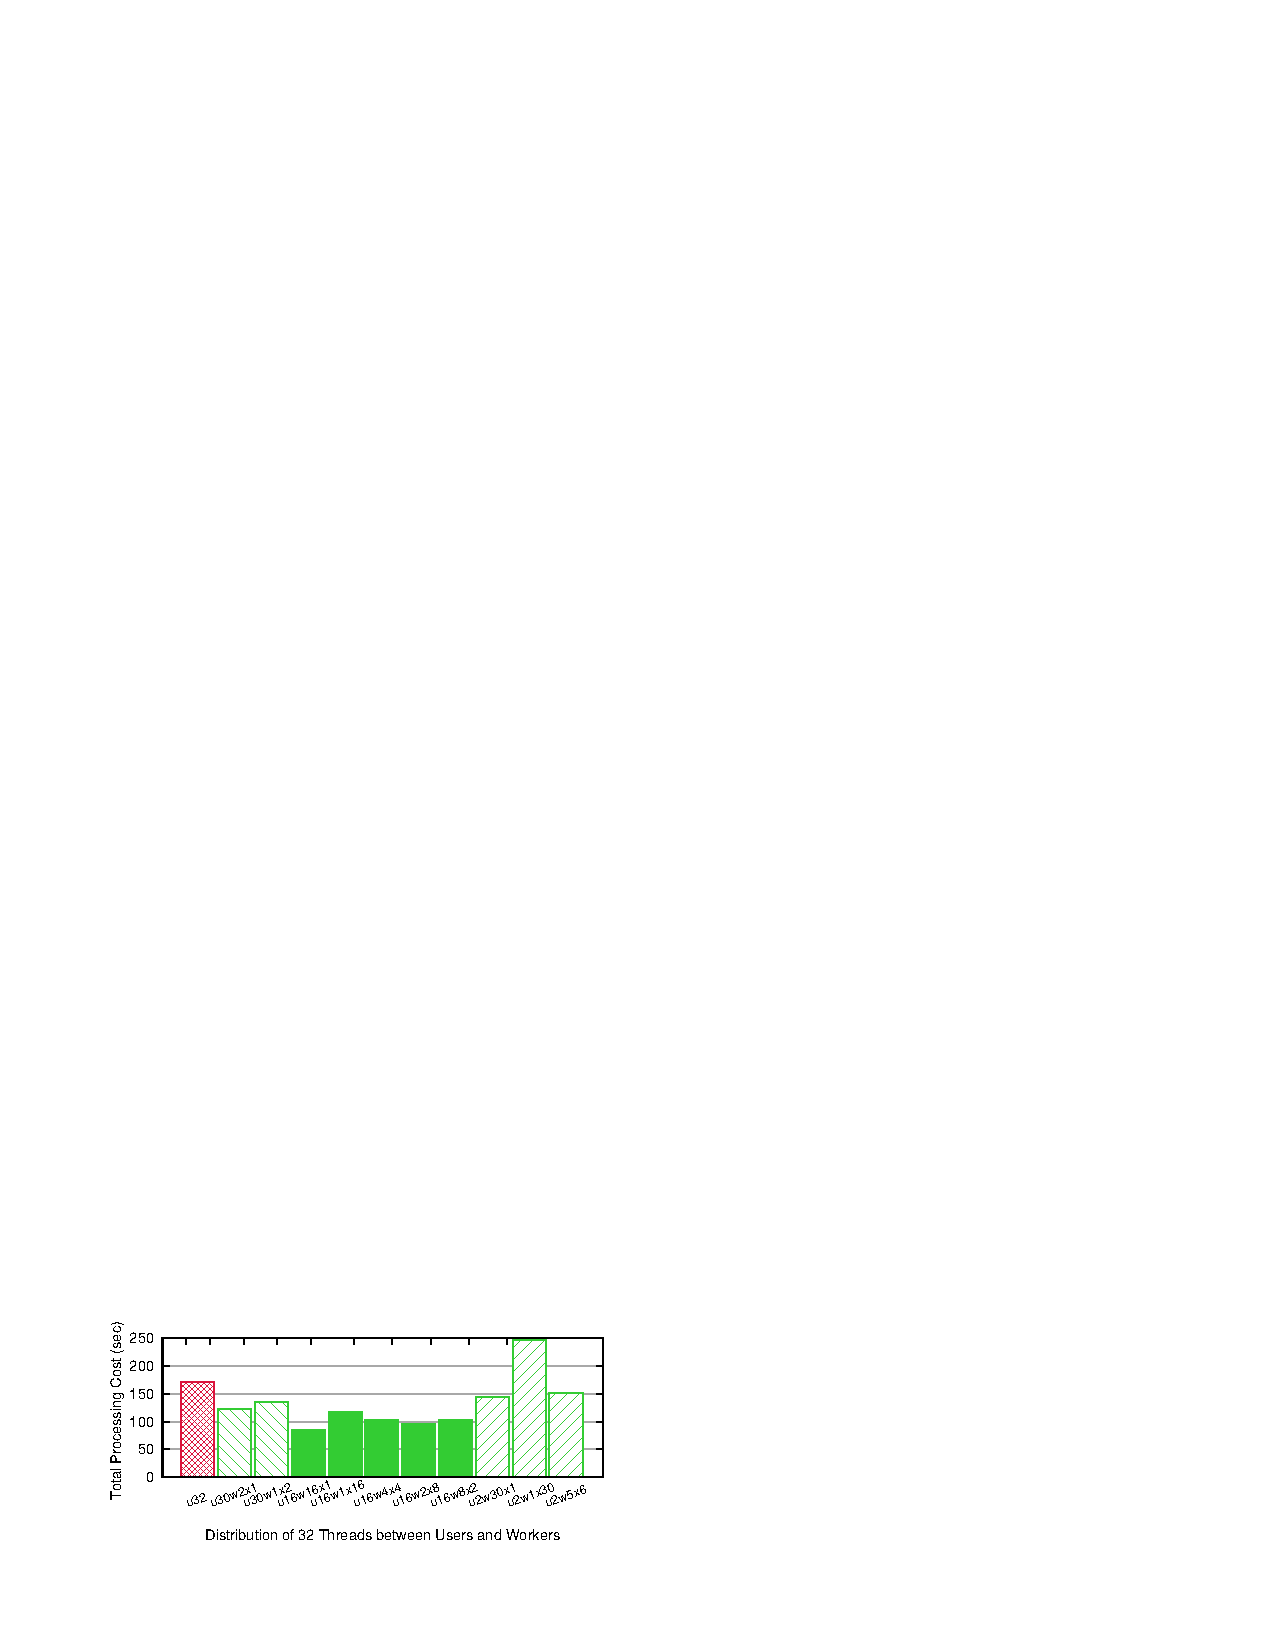
\includegraphics[trim=1.8cm 2cm 0cm 22.3cm]{Figures/holistic/thread_distribution}
\vspace{-0.2 in}
\caption{Performance improves if we distribute the threads equally between user queries and holistic workers.}
\vspace{-0.7 cm}
\label{fig:thread_distribution}
\end{center}
\end{figure}
Holistic indexing manages to further improve the performance of the workload by about 50\%.
Contrary to the other indexing approaches, 
MonetDB with holistic indexing enabled monitors the CPU utilization and constantly  tries to maximize it.
When holistic indexing detects idle CPU resources, it triggers index refinement actions on existing adaptive indices.
In this experiment, an index is inserted in the index set, and specifically in $C_{actual}$, when a user query creates it.
For holistic indexing the actual user queries behave in exactly the same way as in adaptive indexing, i.e., the first
query will create an adaptive index and subsequent queries refine it using the very efficient and almost linearly
scaling parallel vectorized cracking implementation from \cite{efficient_cracking}.
The difference is that with holistic indexing enabled idle CPU resources are exploited towards further refining the adaptive indices
in a way which does not hurt running queries.
Since parallel vectorized cracking \cite{efficient_cracking} is designed to be CPU efficient, encountering only very little resource stalls,
we generated kind of a worst-case scenario for holistic indexing: we limited the maximal
number of hardware context assigned to user queries to 16 (equal to number
of physical cores), leaving at least 16 (otherwise not effectively usable
by the prime user query workload) hardware contexts (``hyper-threads'')
available for holistic indexing.
Constantly, our load-checker usually detects 16 idle hardware contexts, and consequently
starts 8 holistic indexing workers (each using two threads) as shown in
Figure~\ref{fig:motiv}(d). Figure~\ref{fig:thread_distribution} shows that the combination of using maximal 16 (out of
32) hardware contexts for user queries (performing parallel vectorized adaptive indexing \cite{efficient_cracking}), while devoting any
remaining idle hardware context to holistic indexing, improved the overall
performance by a factor 2 over using all 32 hardware contexts for user
queries (and thus none for holistic indexing).


Figure~\ref{fig:motiv}(b) is a breakdown 
of the performance of holistic indexing and adaptive indexing.
The \emph{y}-axis represents the total response time of the first query, the next 9 queries, etc.
The total height of each bar represents the total response time to run the entire workload of $10^3$ queries.
The first few queries do not see any improvement because holistic indexing cannot concurrently refine a column if there are user queries cracking it. 
This is because initially columns have not been 
cracked at all and thus the first few user queries will lock big pieces for cracking. However,
as each column is cracked into smaller pieces, holistic indexing may invoke  actions to refine 
a column even if concurrent queries are cracking it. 
Essentially, each user query needs to lock at most one piece of an adaptive index at a time, i.e., the piece it is about to crack,
and thus holistic indexing may choose any of the remaining pieces to perform further index refinements.

Holistic indexing outperforms adaptive indexing by a factor 2 by injecting additional index refinements on top of those that adaptive indexing does anyway.
Figure~\ref{fig:motiv}(c) shows the amount of pieces which have been created in all 10 adaptive indices; holistic 
indexing creates more pieces than adaptive indexing. 
As a result, 
future
\begin{wrapfigure}{l}{0.166\textwidth}
\begin{center}
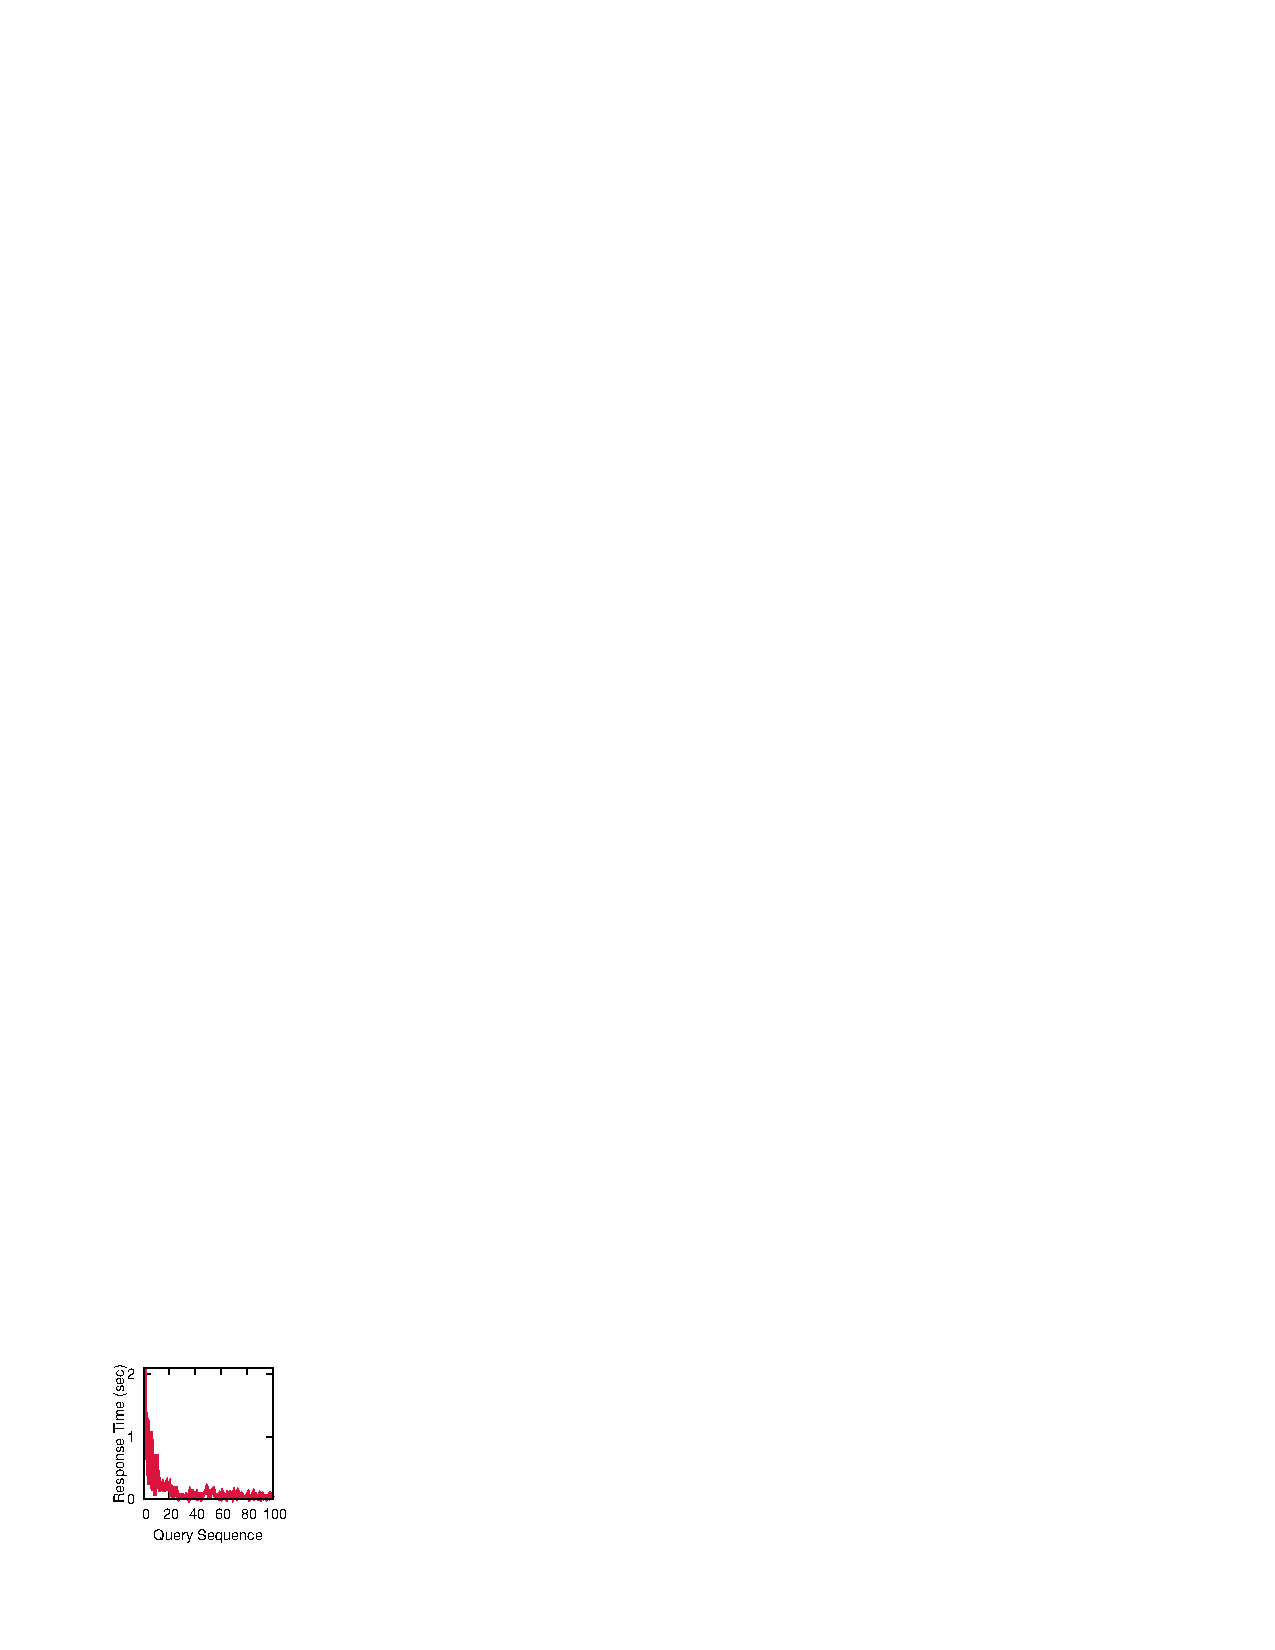
\includegraphics[trim=2.9cm 2cm 18.5cm 23.7cm]{Figures/holistic/cost_graph}
\vspace{-0.1in}   %-0.1in
\caption{\small{Adaptive Ind.}}
\vspace{-0.7cm}
\label{fig:cost_graph}
\end{center}
\end{wrapfigure}
 user queries need to touch less data as they find a fine-grained index, and thus performance improves for holistic indexing. As Figure~\ref{fig:cost_graph}
 shows, the first queries that access the same index run slower, because they reorganize big partitions. Thus, additional
pieces have to be inserted in the index as early as possible in the query sequence.


As discussed in Section~\ref{subsec:design}, on some occasions 
the main holistic indexing thread waits for all workers to finish before assigning new tasks,
leaving under-utilized CPU resources for some brief periods. 
Figure~\ref{fig:motiv}(d) shows how the total response time 
of all workers in every tuning cycle changes over time and as the  query sequence evolves.
The right $y$-axis shows the number of holistic worker threads the holistic indexing thread activates whenever it detects idle CPU resources.
The maximum number of workers that holistic indexing can activate is 8. %, i.e., equal to the number of cores in our system.
The left $y$-axis represents the total response time of all workers during a single tuning cycle. 
The $x$-axis represents the activations  of holistic indexing.
A single activation of holistic indexing triggers the activation of multiple holistic workers.
The total response time of the workload is 90 seconds.
Within this amount of time, holistic indexing is activated only 15 times, because of the waiting time (1 second) between two CPU load measurements and because of the waiting time until all workers finish in every tuning cycle.
We observe that the response time of the workers is high only for the first few activations and reduces very fast as the index becomes fine-grained. In this way, the system adapts on its own and eventually no worker is a bottleneck.

Holistic indexing sees even bigger performance benefits when there is idle time before query processing.
When there is idle time and no workload knowledge, holistic indexing chooses random indexes to insert in $C_{potential}$  and refines them until the first query arrives. Here using the same set-up as in the previous experiment, we manually induce idle time and holistic indexing adds 10 random indices in $C_{potential}$ .
Figure~\ref{fig:apriori} shows the results.
Compared to adaptive indexing, which does not exploit the a priori idle time
\begin{wrapfigure}{l}{0.166\textwidth}
\begin{center}
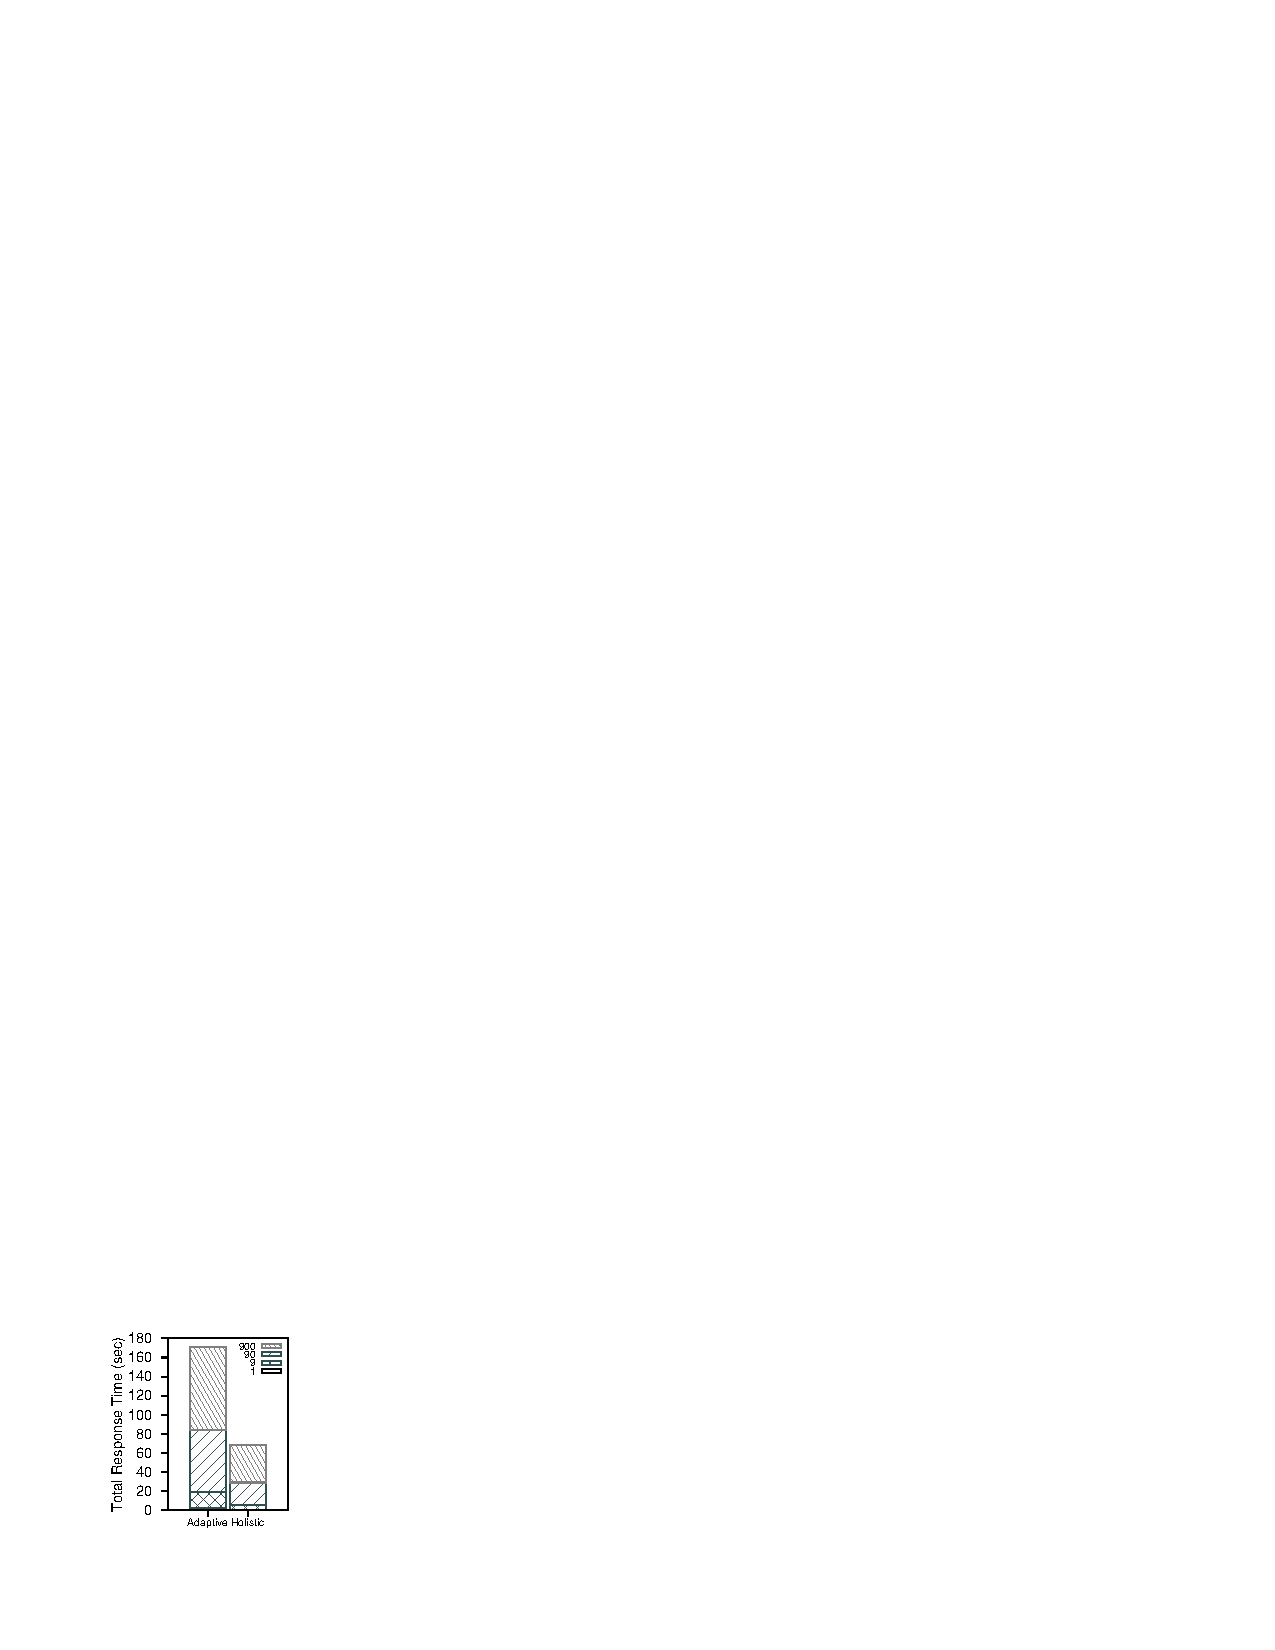
\includegraphics[trim=2.8cm 1.8cm 18cm 23cm]{Figures/holistic/hist_motivation_apriori}
\vspace{-0.2in}
\caption{Indexing.}
\vspace{-0.7cm}
\label{fig:apriori}
\end{center}
\end{wrapfigure}
e (22 seconds), holistic indexing exploits 
this time to spread tuning actions over 10 indices.
Thus, when user queries are processed they reorganize smaller partitions and the benefit is already obvious in the beginning of the workload compared to Figure~\ref{fig:motiv}(b), where the benefit in the workload appears after the 10th query when all indices have been inserted in the index set automatically by the system.

By being able to completely automatically utilize available CPU resources and direct them 
towards lightweight actions that may improve future requests,
holistic indexing can bring significant performance gains on top of existing indexing approaches. 
It outperforms adaptive indexing by a factor 2 in terms of individual query performance
At the same time it outperforms offline and online indexing, especially in the beginning of the workload, 
when offline indexing penalizes the first queries with the index building cost and online indexing does not provide any indexing support
until the 100th query.
Besides the difference in performance, the qualitative difference described in Table~\ref{tab:qualitative}, makes holistic indexing a very appealing indexing approach in modern dynamic environments.

%\vspace{-0.2 in}

\begin{figure*}[t]
     \begin{center}

        \subfloat[Random]{%
            \label{fig:random_pred}
            
\includegraphics[trim=2cm 2cm 16.3cm 24cm]{Figures/holistic/random_predicates}
        }%
	\subfloat[Skewed]{%
            \label{fig:skew_pred}
            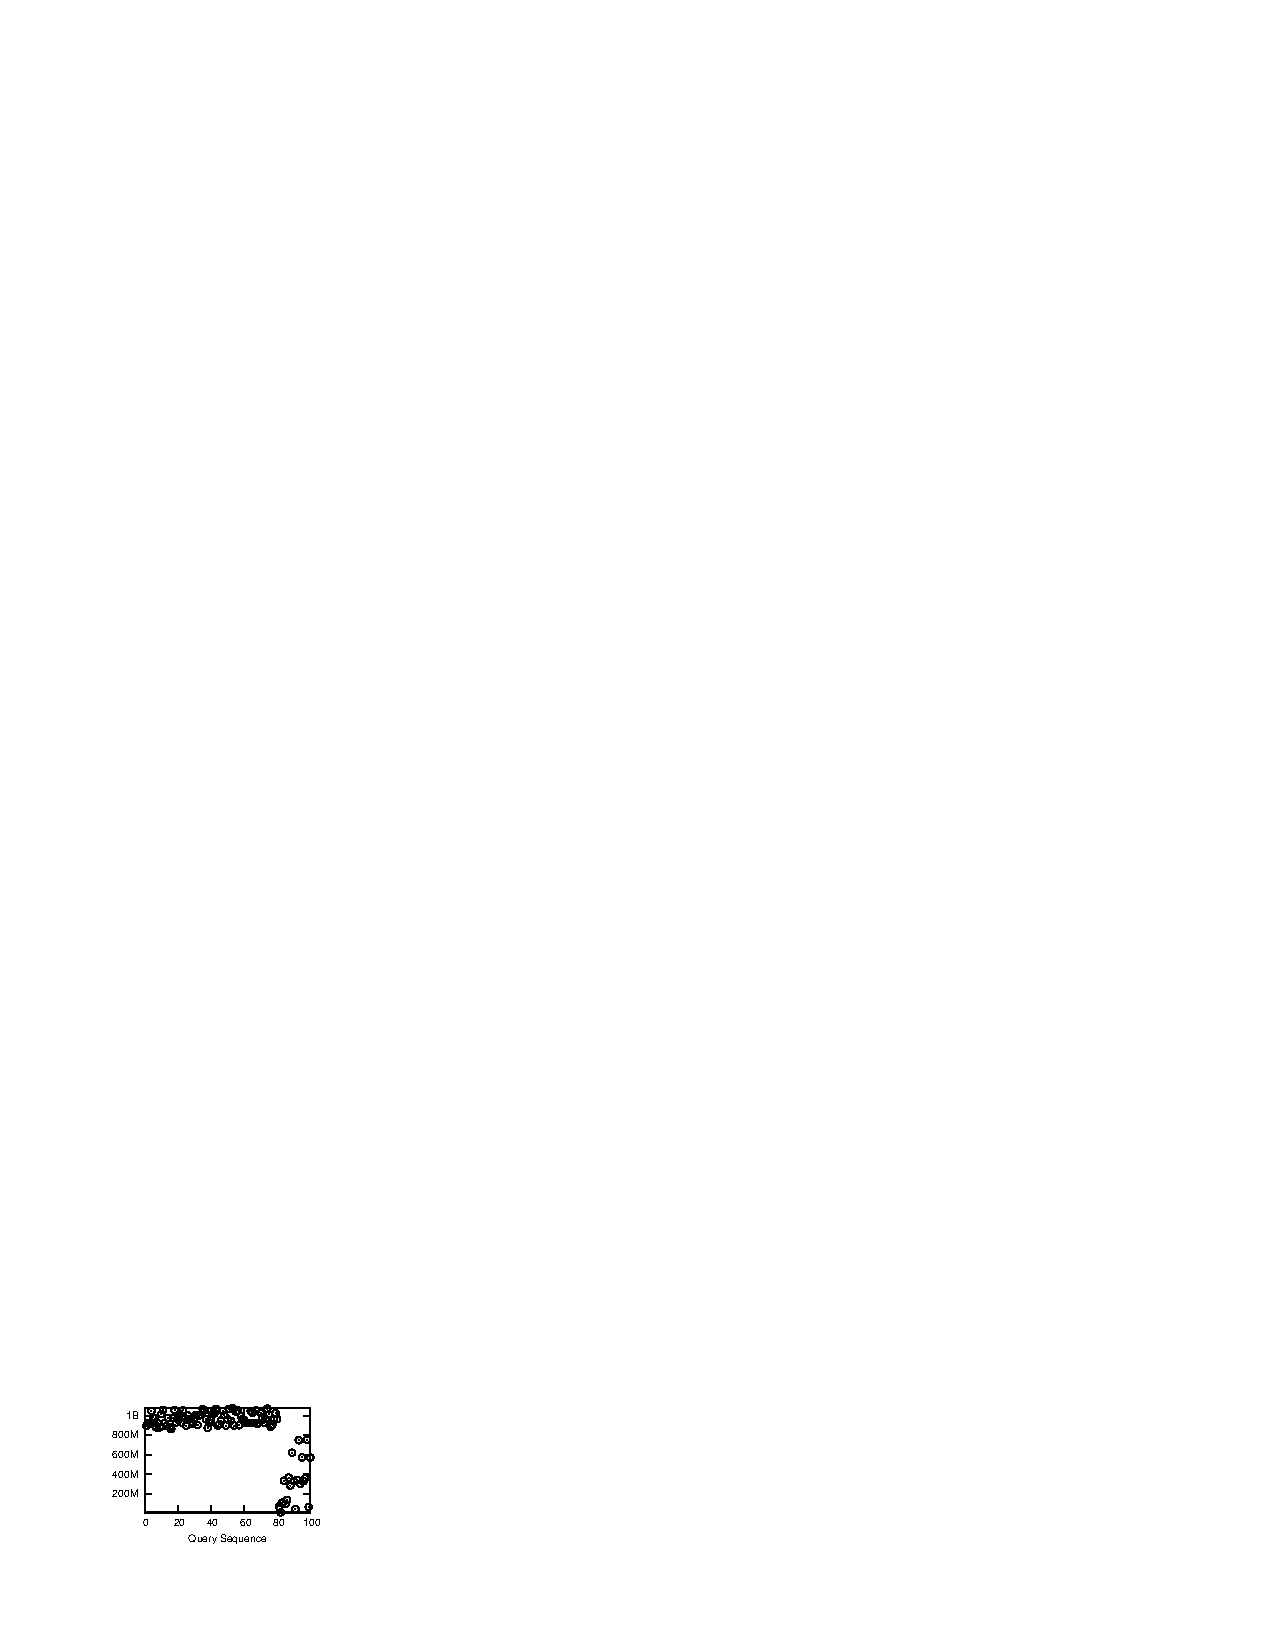
\includegraphics[trim=2cm 2cm 16.3cm 24cm]{Figures/holistic/skew_predicates}
        }%
      \subfloat[Periodic]{%
           \label{fig:periodic_pred}
           
\includegraphics[trim=2cm 2cm 16.3cm 24cm]{Figures/holistic/periodic_predicates}
        }%
       \subfloat[Sequential]{%
            \label{fig:sequential_pred}
            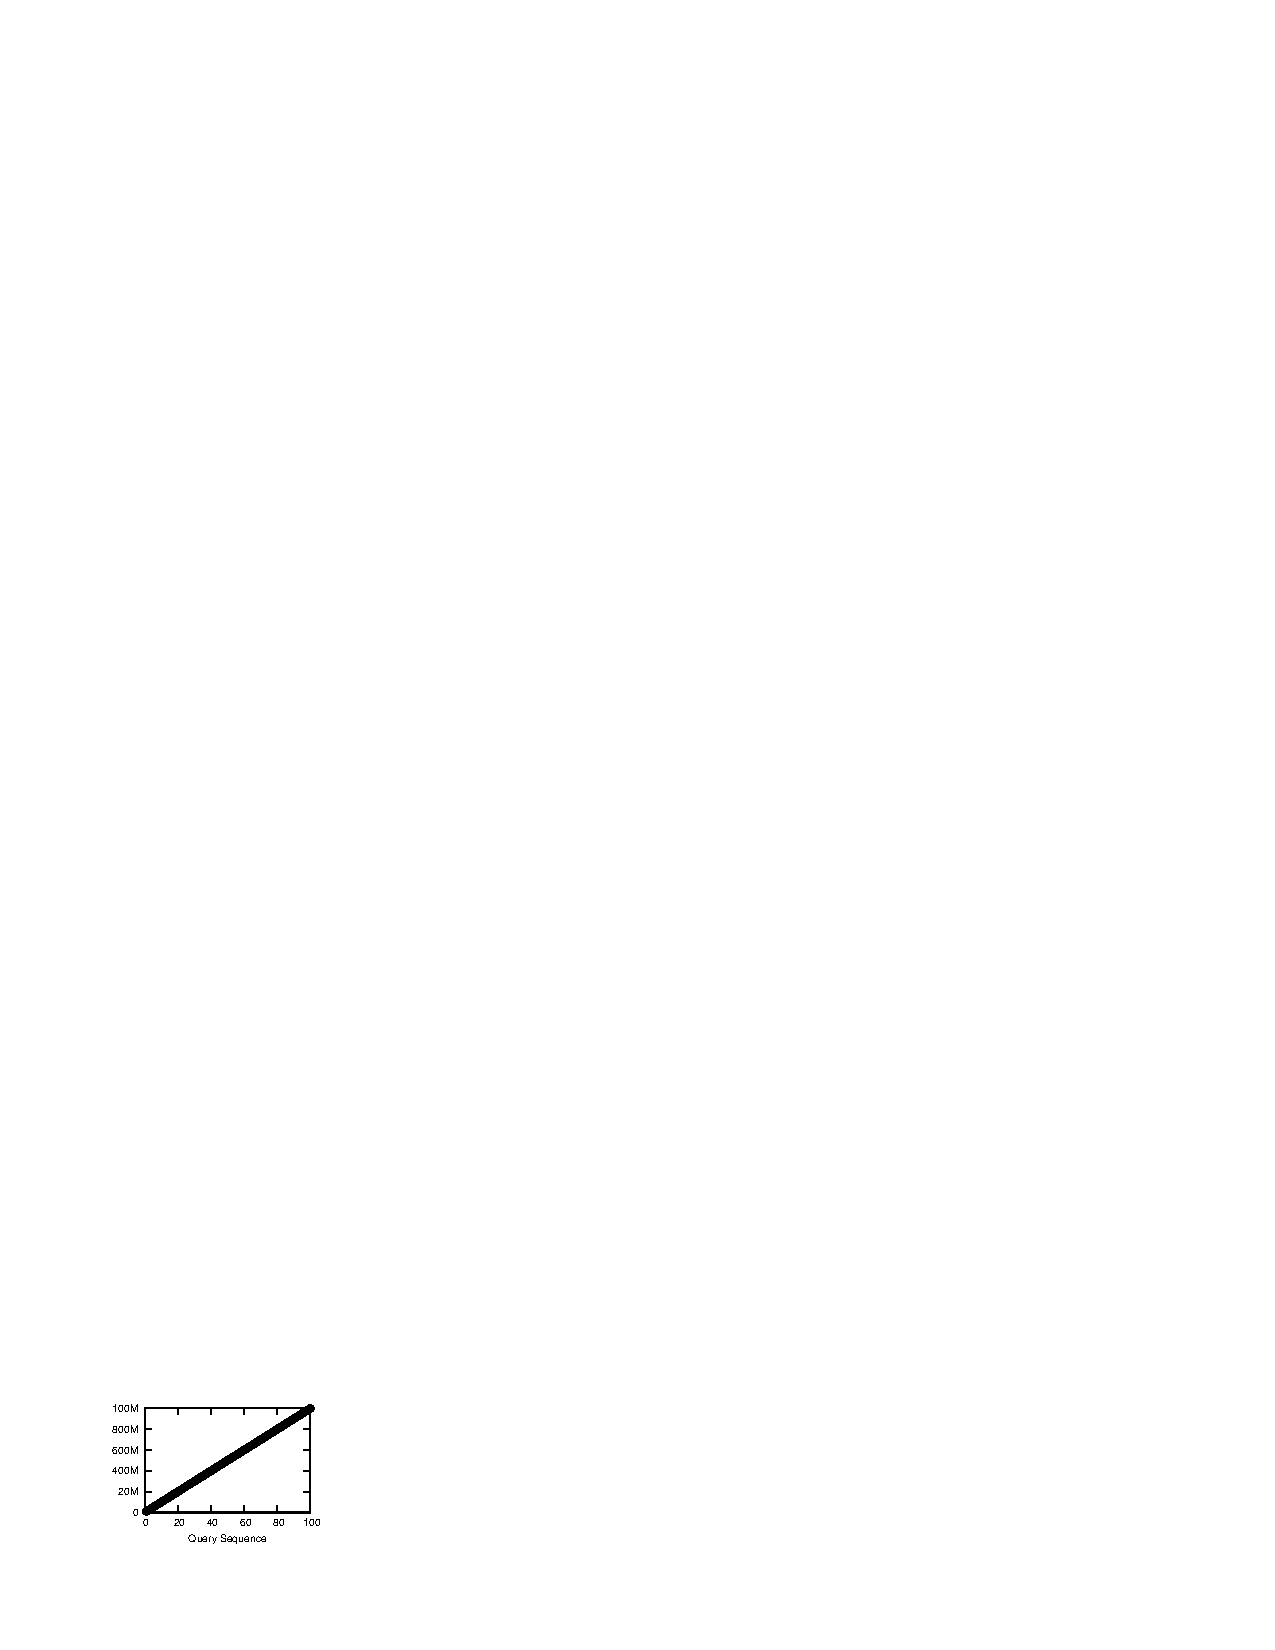
\includegraphics[trim=2cm 2cm 16.3cm 24cm]{Figures/holistic/sequential_predicates}
        }%
       \subfloat[SkyServer]{%
            \label{fig:sequential_pred}
            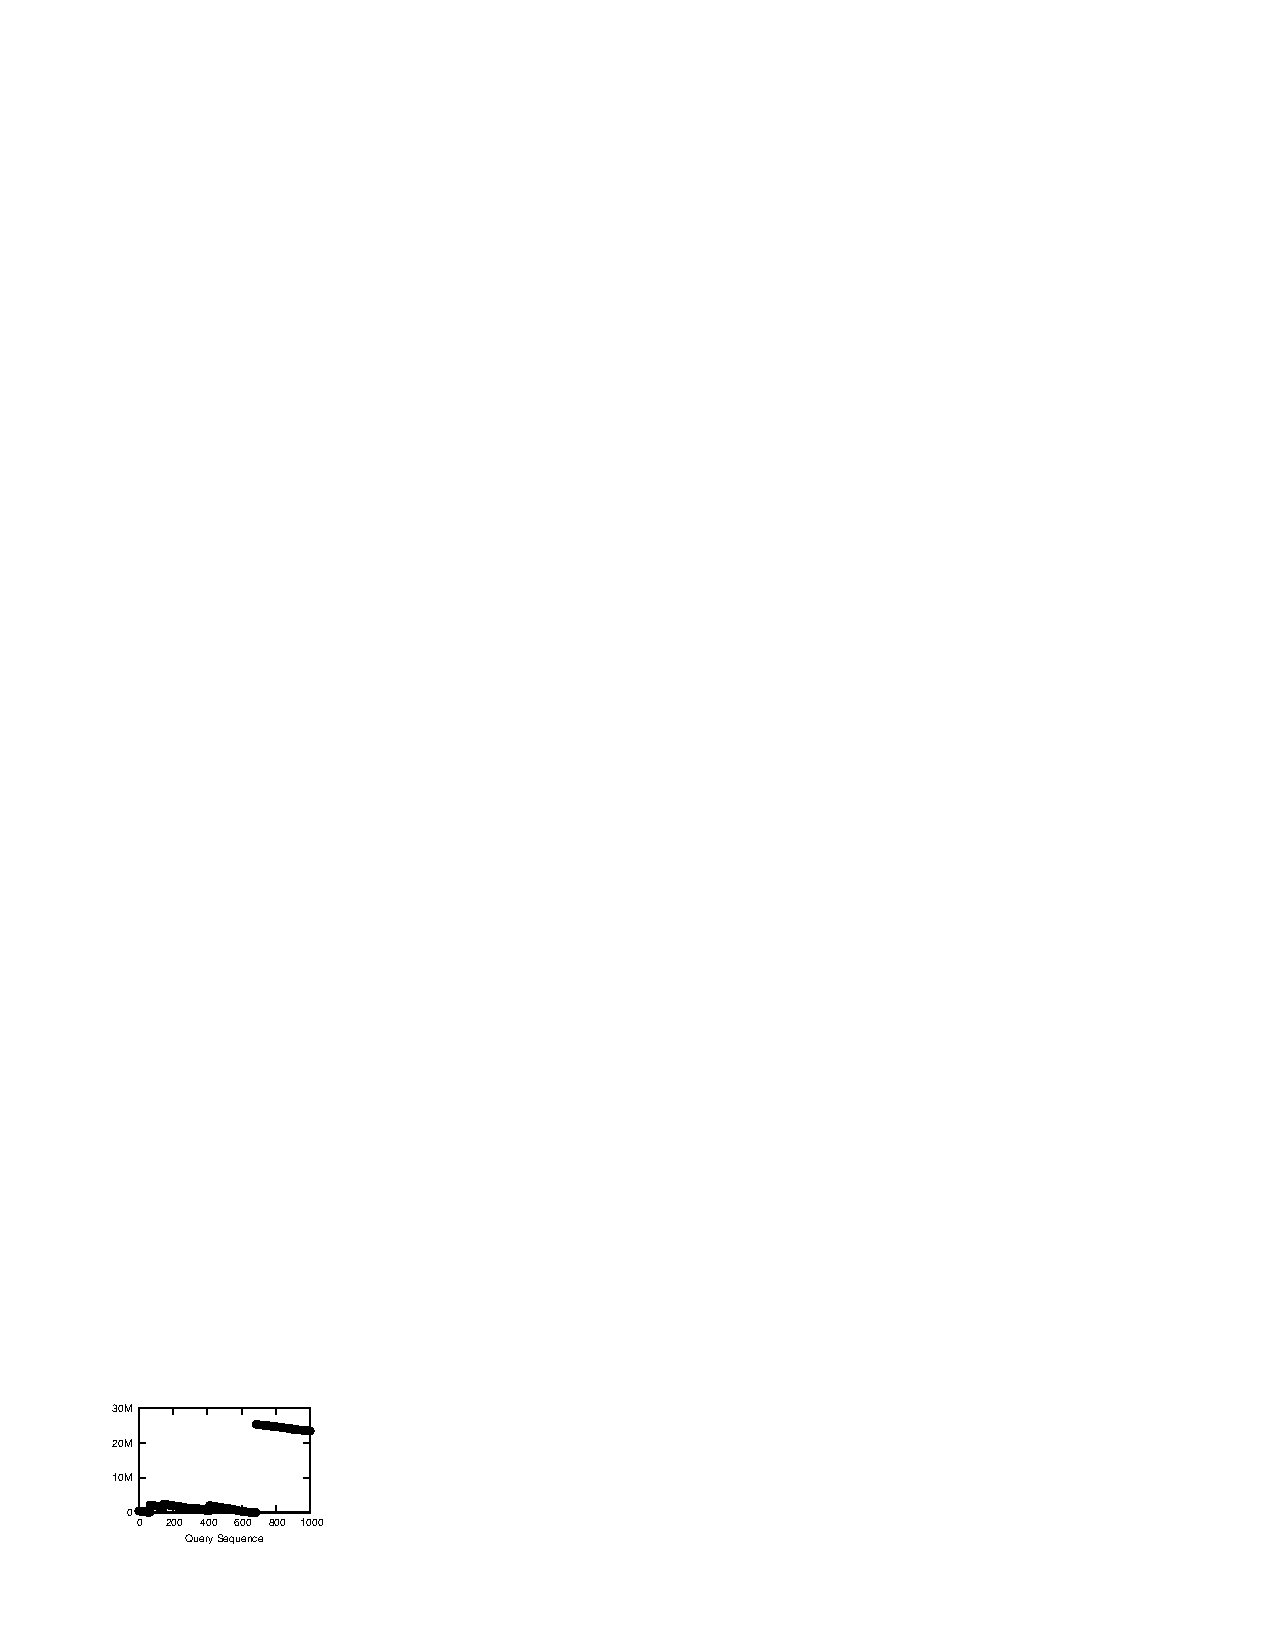
\includegraphics[trim=2cm 2cm 16.3cm 24cm]{Figures/holistic/skyserver_predicates}
        }%
\vspace{-0.25 in}
    \caption{Various workload patterns.}
\vspace{-0.7 cm}
   \label{fig:rob1}
    \end{center}
\end{figure*}

\begin{figure}[!htb]
\begin{center}
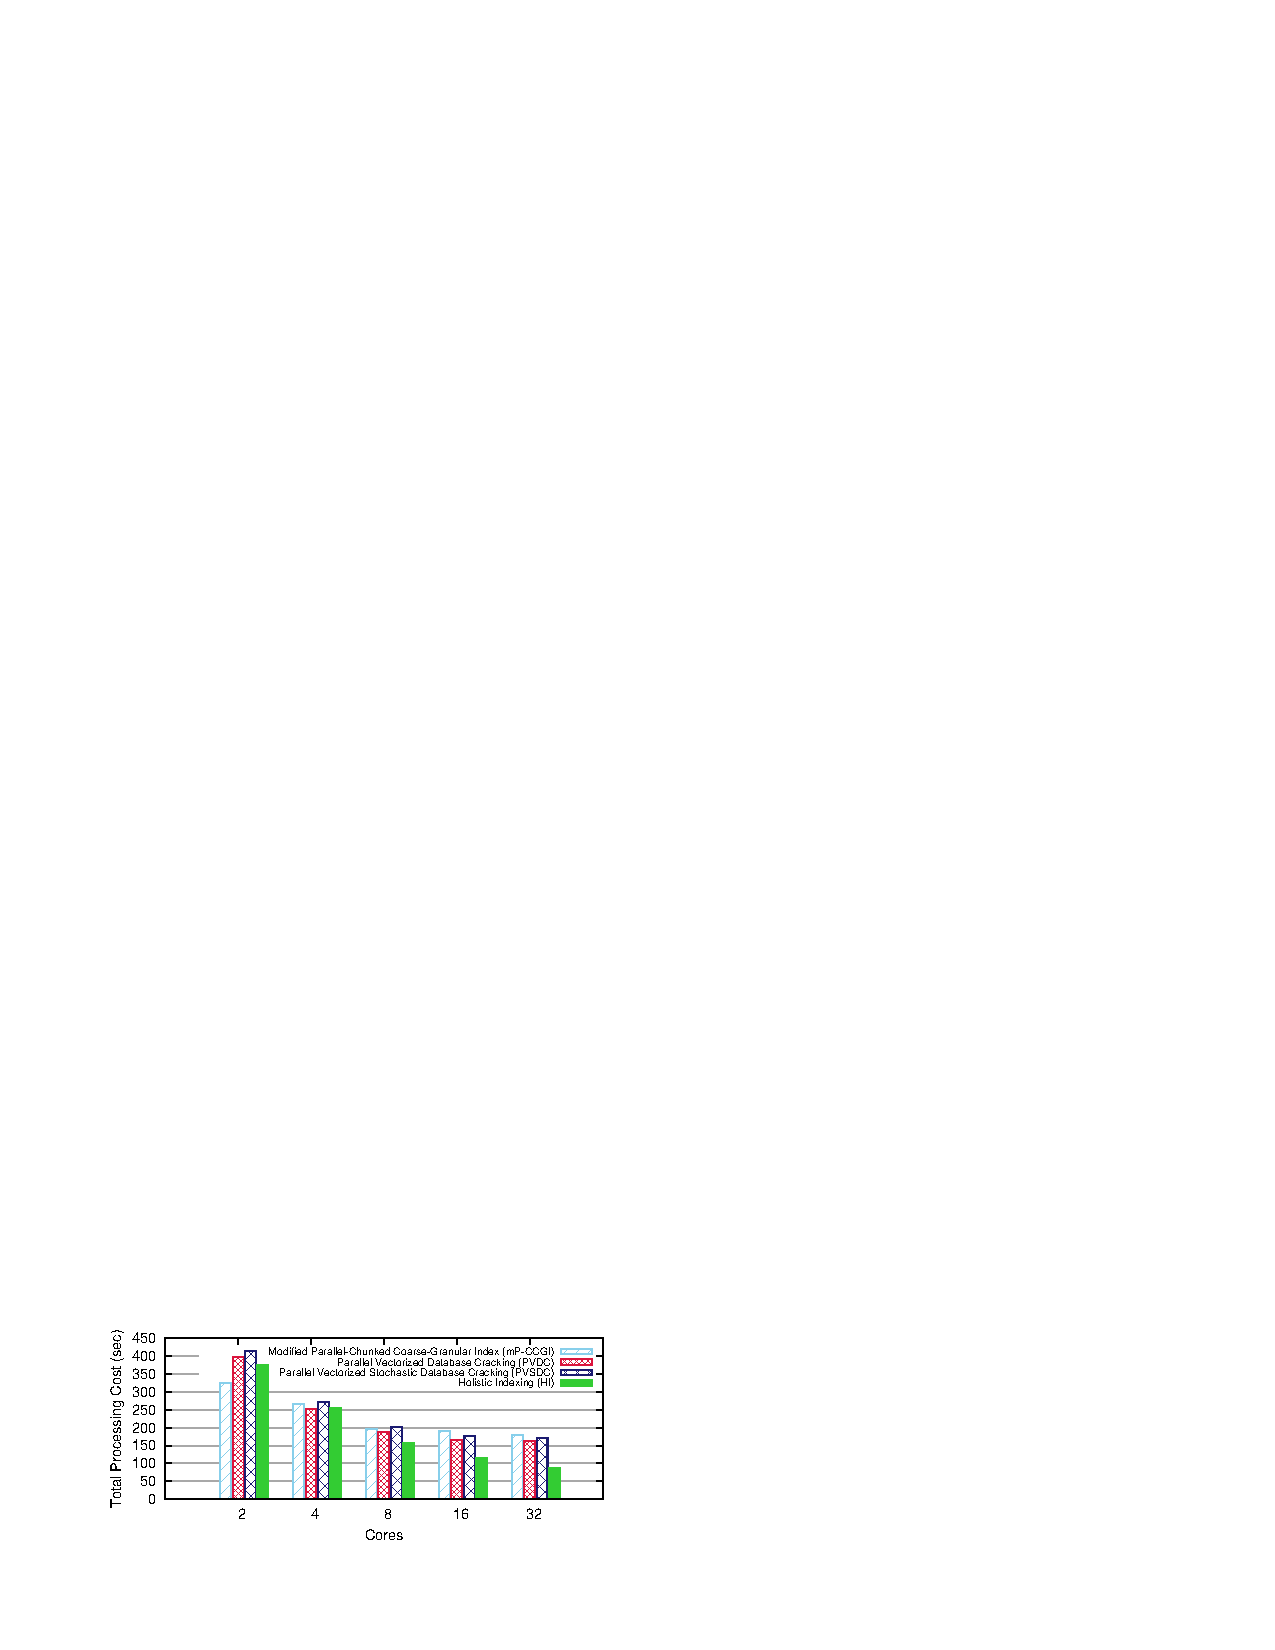
\includegraphics[trim=1.8cm 2cm 0cm 22.4cm]{Figures/holistic/multicore}
\vspace{-0.25 in}
\caption{Holistic indexing utilizes resources more effectively than multi-core state-of-the-art adaptive indexing baselines.}
\vspace{-0.7 cm}
\label{fig:multicore}
\end{center}
\end{figure}


\subsection{Holistic Vs. Multi-core Adaptive Indexing}
\label{subsec:multicore}

Assuming there are  several CPU cores available in a modern system, 
in holistic indexing we utilize them by spreading auxiliary tuning actions across multiple indices.
An alternative way to ``keep the CPU busy'', is to parallelize the existing adaptive indexing algorithms.
In this experiment we study how state-of-the-art adaptive indexing baselines compare to holistic indexing. In particular, we study parallel vectorized database cracking (PVDC), parallel vectorized stochastic database cracking (PVSDC) \cite{efficient_cracking} and a modified version of parallel chunked coarse granular index (P-CCGI) \cite{multicore_adaptive} that we name mP-CCGI.

Stochastic cracking aims to provide robustness by performing auxiliary stochastic indexing actions.
Although stochastic cracking studied the option of collecting statistics to target the proper value ranges to index, 
it was shown in \cite{DBLP:journals/pvldb/HalimIKY12} that reacting immediately to workload changes by auxiliary 
stochastic cracking actions has a better effect (i.e., more robust).
This is because in stochastic cracking a running query performs auxiliary random cracking only within the piece that is already about to be cracked
within a given column and as a result any action brings a benefit as it imposes more order. Holistic indexing considers a much more broad space of statistics
keeping track of column-statistics to decide which columns to fine tune. 

Both stochastic cracking and plain database cracking in this experiment utilize 
multi-cores as described in the last paragraph of Section~\ref{sec:problem}.
The original P-CCGI algorithm partitions the data into as many chunks as the available number of threads and 
the first query cracks each chunk in parallel having a separate cracking index for each chunk.
Subsequent queries crack the chunks in parallel, while they benefit from the initial range partitioning.
However, this way, data that belongs in a single value range is physically stored in separate chunks/arrays 
and feeding from there other relational operators is not compatible with a column-store such as MonetDB  that relies on bulk processing;
it does not allow to exploit tight for loops without intermediate if statements to detect when we should skip from one chunk to the next during an operator. 
To address this we extended the original P-CCGI algorithm \cite{multicore_adaptive} with the ability to consolidate selection results in a single array
using the same techniques that were used for hybrid adaptive indexing which also operates on multiple chunks (but not in parallel) 
\cite{DBLP:journals/pvldb/IdreosMKG11}; each query
consolidates only the qualifying value ranges and each value range needs to be written to the contiguous array by a single query only, 
i.e., subsequent queries will only have to do consolidation if they need a new value range never consolidated before.
In a vectorized column-store this could be done without consolidation, potentially improving performance further
as has been indicated by partial sideways cracking \cite{DBLP:conf/sigmod/IdreosKM09};
vectorized processing for adaptive indexing is an open topic, though, orthogonal to this work.

The workload in this experiment consists of 10$^{3}$ select-project queries (as in the previous experiment) on 10 integer attributes.
Each attribute consists of 2$^{30}$ uniformly distributed integers.
The value range requested by each query is random while we vary
the number of available CPU cores from 2 to 32, i.e., the maximum number of cores in our system.
For holistic indexing we give half of the cores to user queries  and the rest of the cores are used by the workers (after testing all possible configurations, we found that this is the one that performs best in all cases).
The labels on top of the bars that represent the performance of holistic indexing indicate the distribution of the threads between user queries and workers in every case
(similar to Figure~\ref{fig:thread_distribution}).




Figure~\ref{fig:multicore} shows the results.
In all cases, the performance improves as we invoke more cores into query processing.
For multi-core database cracking and stochastic cracking the performance improves because many threads crack in parallel for one query at a time
while for holistic indexing performance improves because many threads work in the background in parallel with query processing
to further refine the various indices with auxiliary indexing actions.
Holistic indexing sees a bigger improvement, because it is active all the time, i.e., maximizing CPU usage.%every time it drops.
 On the contrary, multi-core vectorized database cracking and multi-core stochastic cracking improve the performance only during user queries and only during the cracking actions.
Another subtle difference but one with a major performance impact is that while stochastic cracking and database cracking target all their adaptive indexing
 actions on specific pieces as they are driven by individual queries, holistic indexing spreads its actions across the whole range of the
domain and thus across the whole range of an adaptive index (stochastic cracking does random actions but only within a single piece). 
This creates a nicely balanced index which has more potential to benefit future queries.
The modified version of P-CCGI initially range partitions the data, which can be seen as a pre-index step. 
However, this is a cost that penalizes the first set of queries.


\begin{figure}[!htb]
\begin{center}
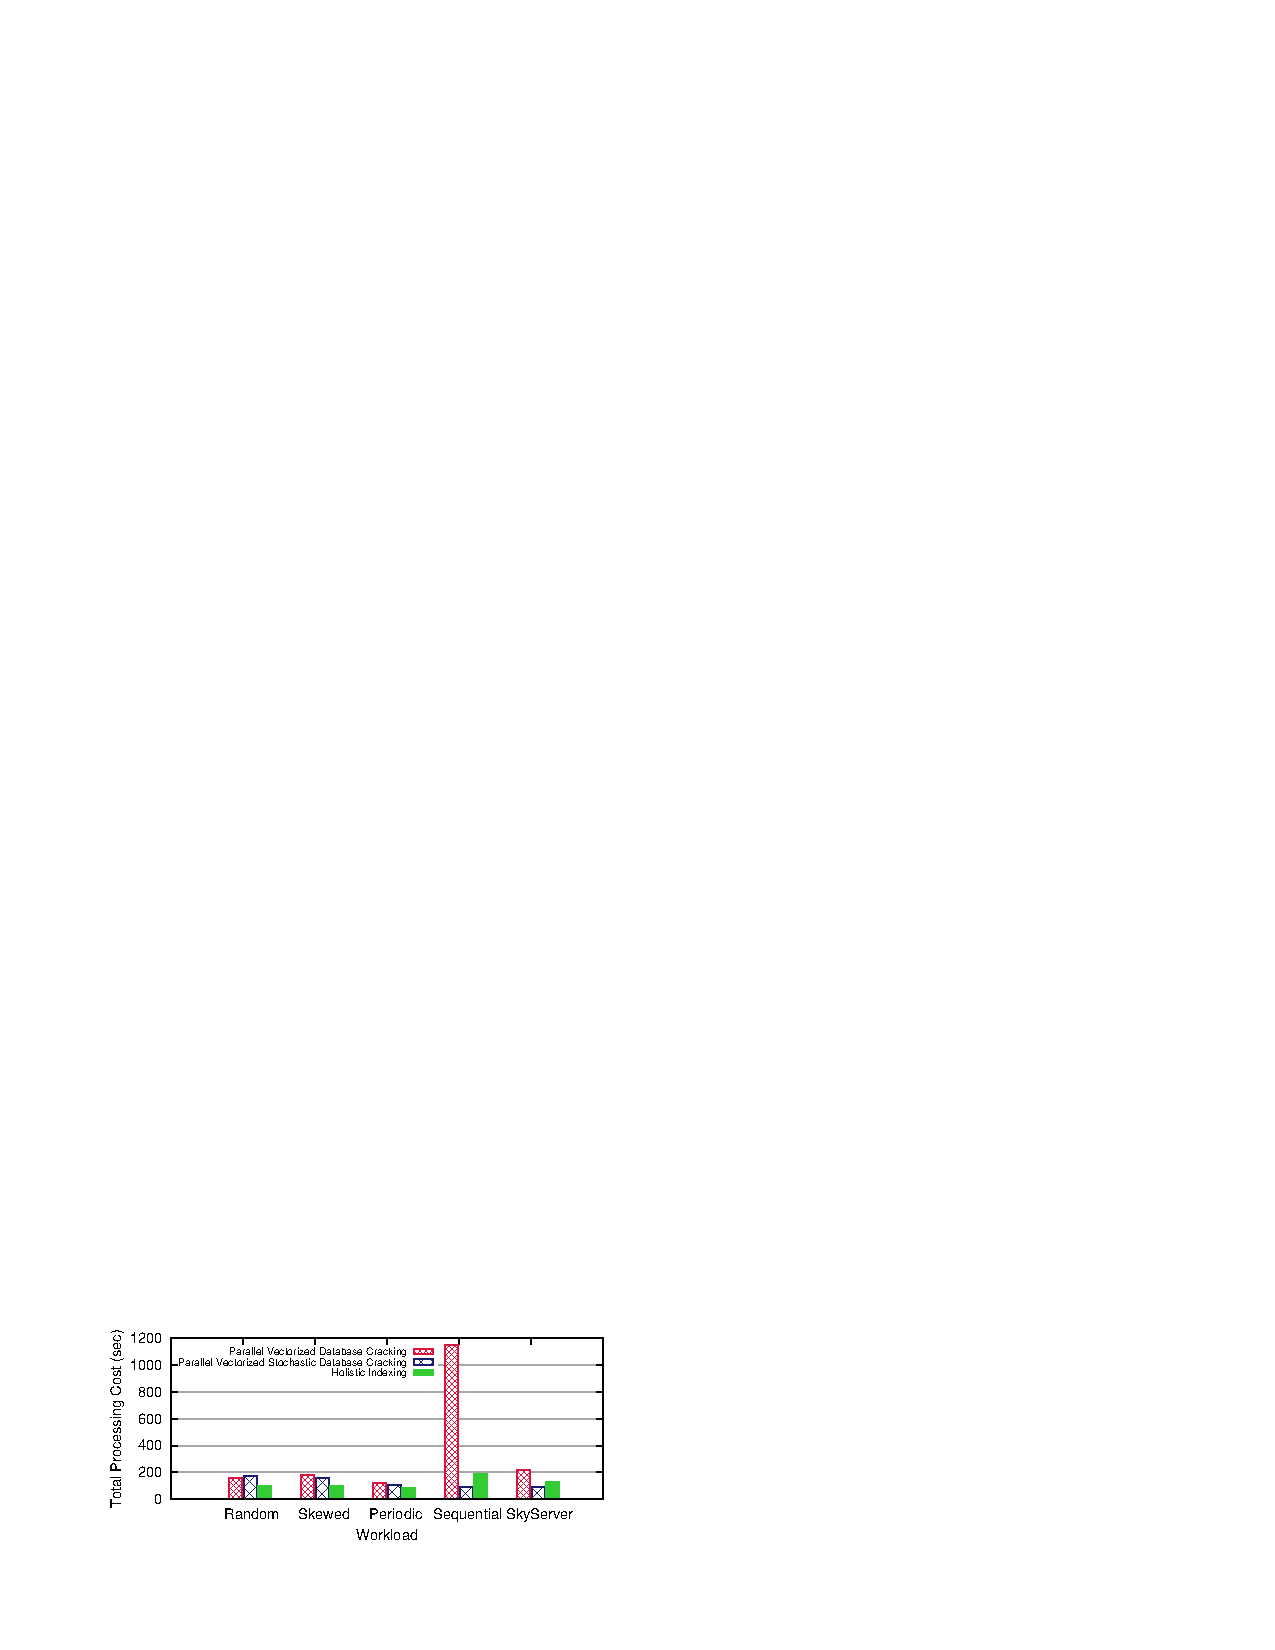
\includegraphics[trim=1.8cm 2cm 0cm 22.8cm]{Figures/holistic/sev_workloads}
\vspace{-0.25 in}
\caption{Holistic indexing is robust.}
\vspace{-0.7 cm}
\label{fig:stochastic}
\end{center}
\end{figure}


\begin{figure*}[ht]
     \begin{center}

        \subfloat[Random Attributes - Random Values]{%
            \label{fig:random_ma}
            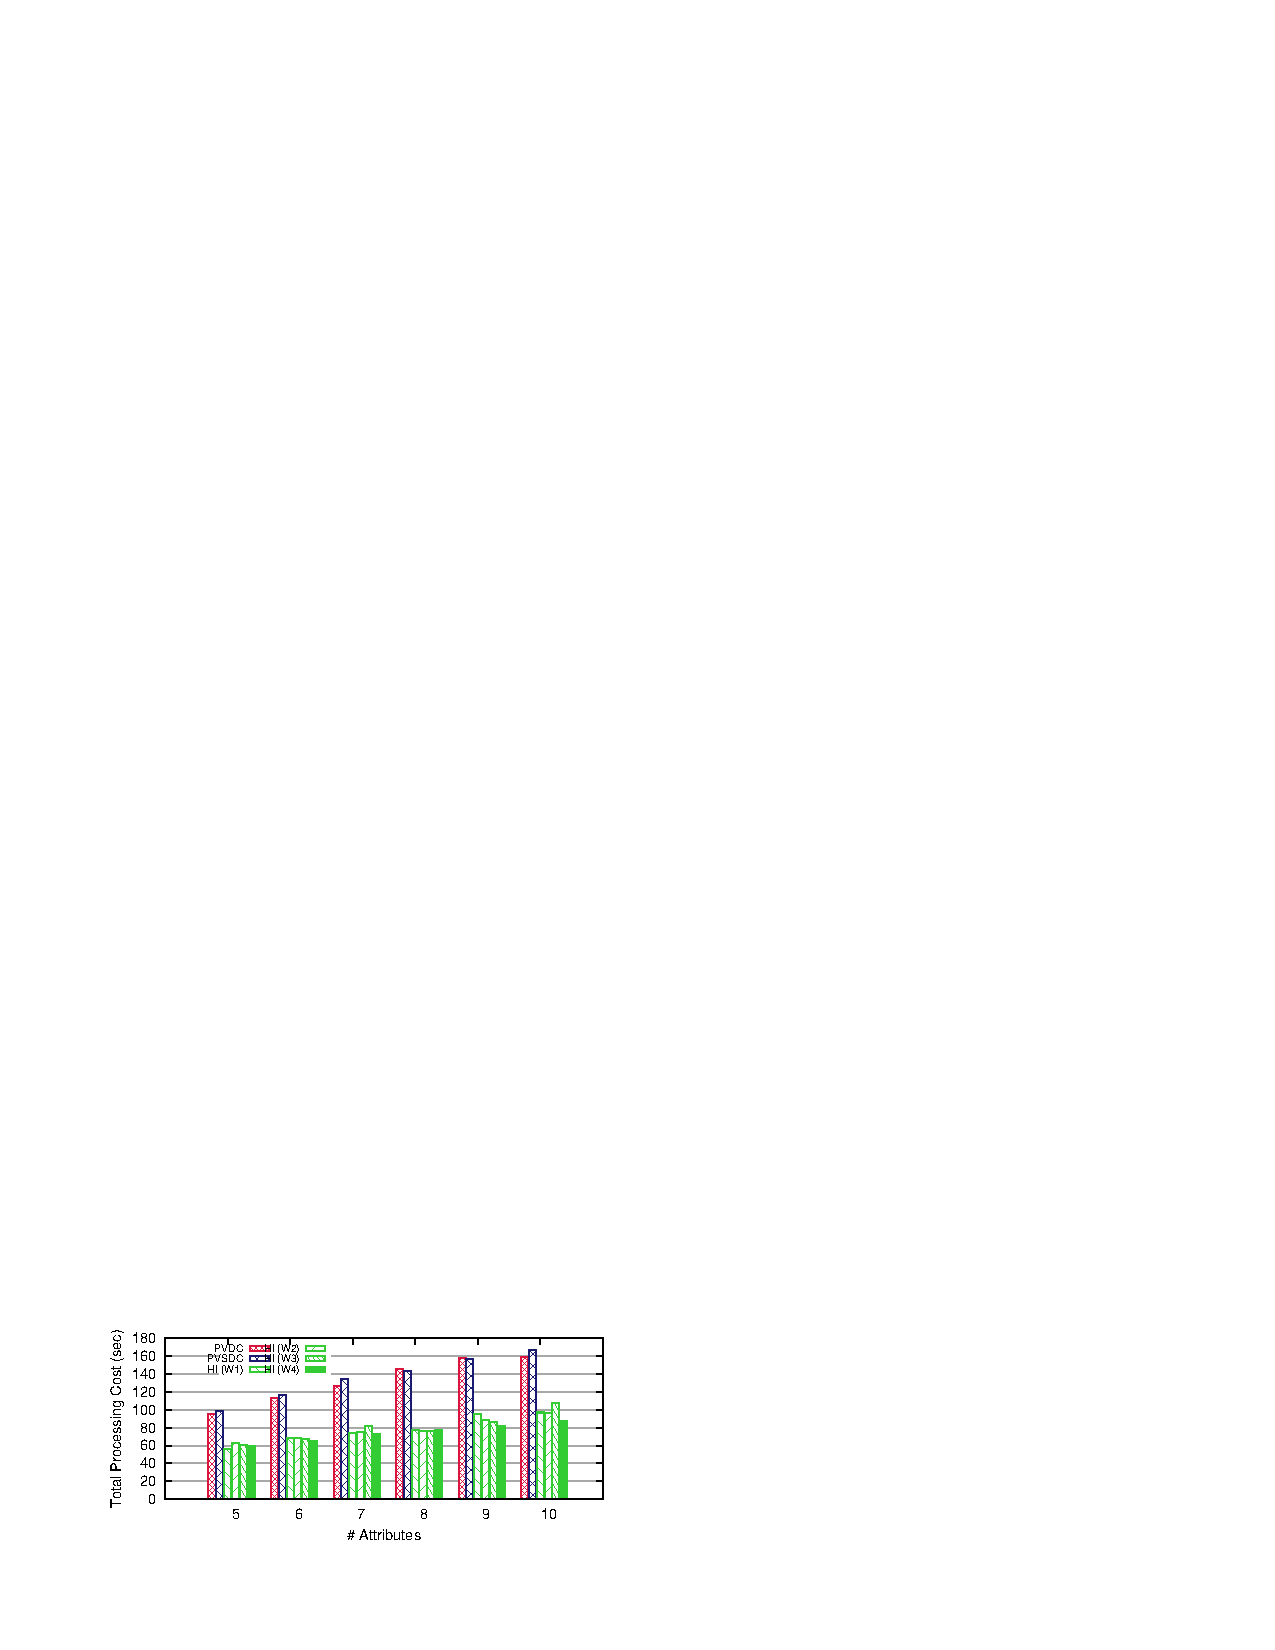
\includegraphics[trim=1.8cm 2.2cm 11cm 23cm]{Figures/holistic/random_ma}
        }\vspace{-0.1 in}%
	\subfloat[Random Attributes - Periodic Values]{%
            \label{fig:random_per_ma}
            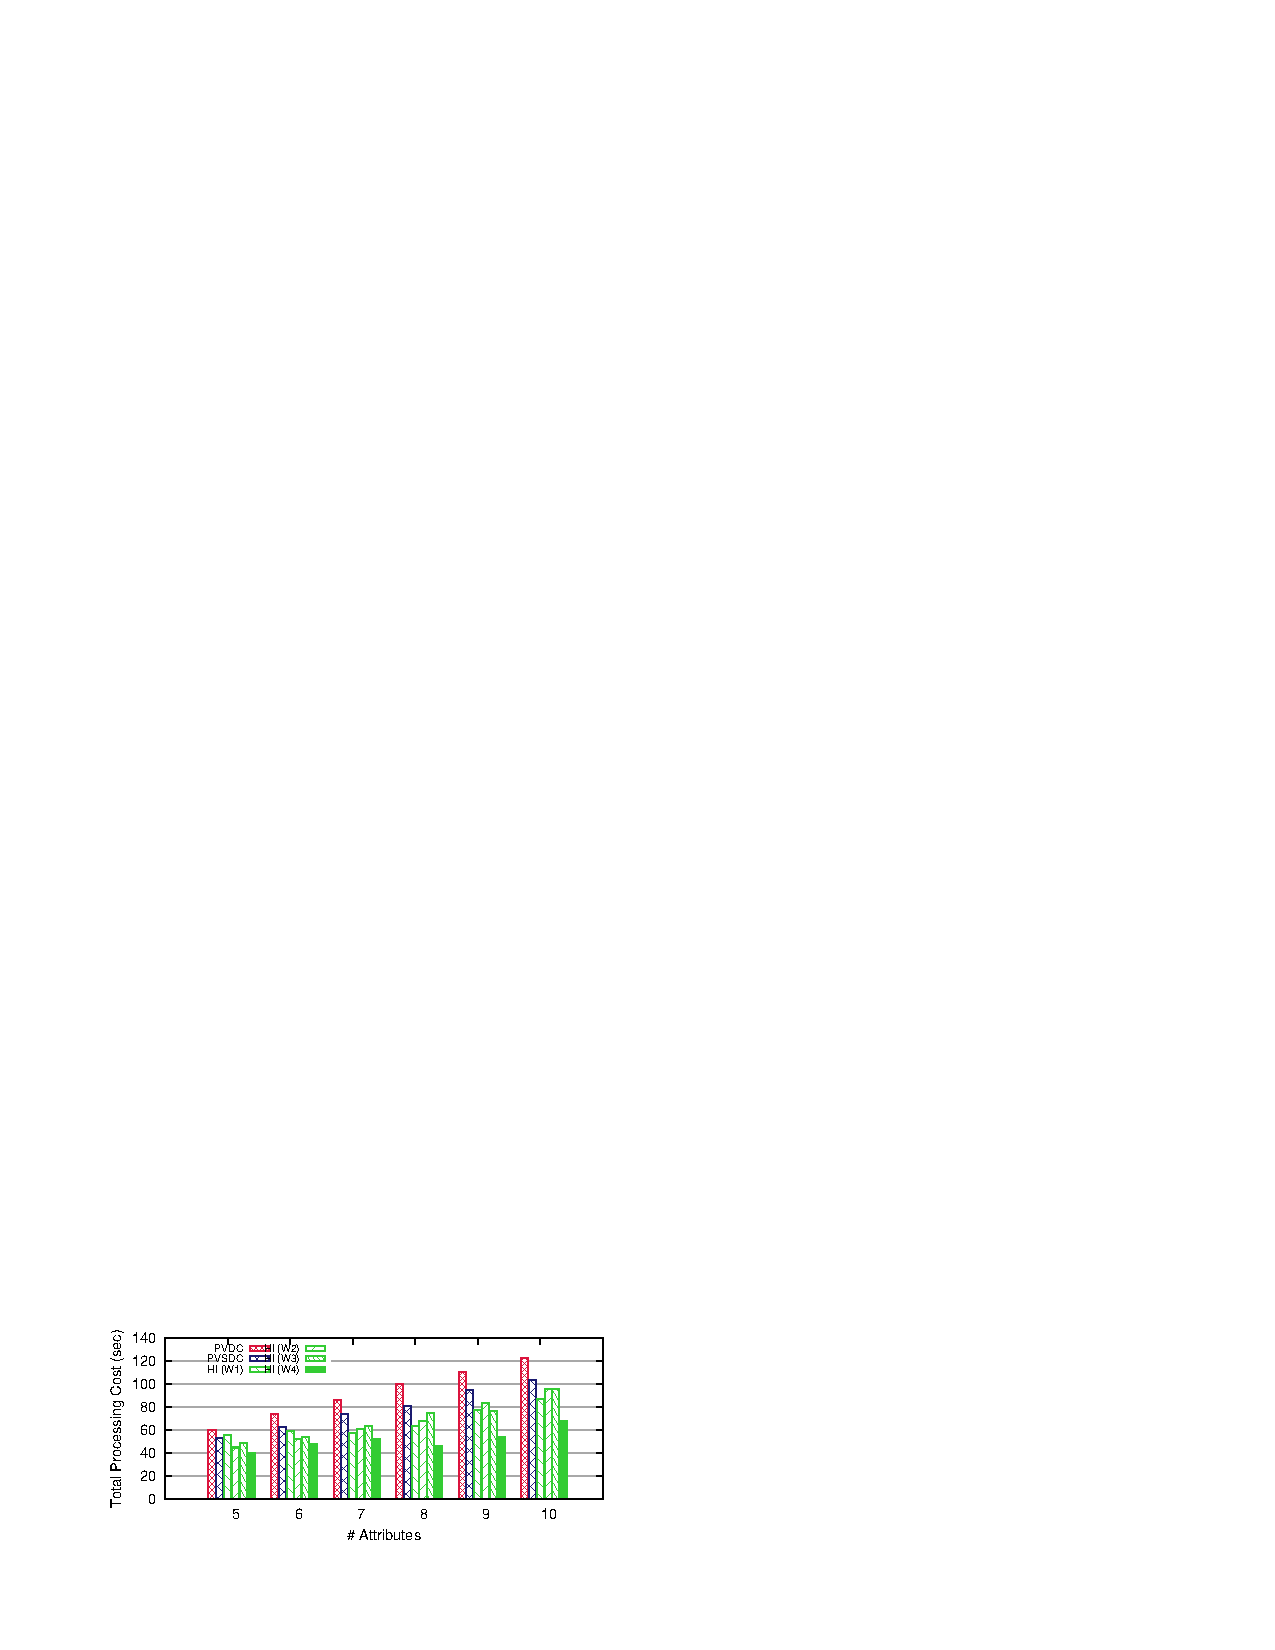
\includegraphics[trim=1.8cm 2.2cm 11cm 23cm]{Figures/holistic/random_per_ma}
        }\vspace{-0.45 in}\\%
	 \subfloat[Skewed Attributes - Random Values]{%
            \label{fig:skew_ma}
            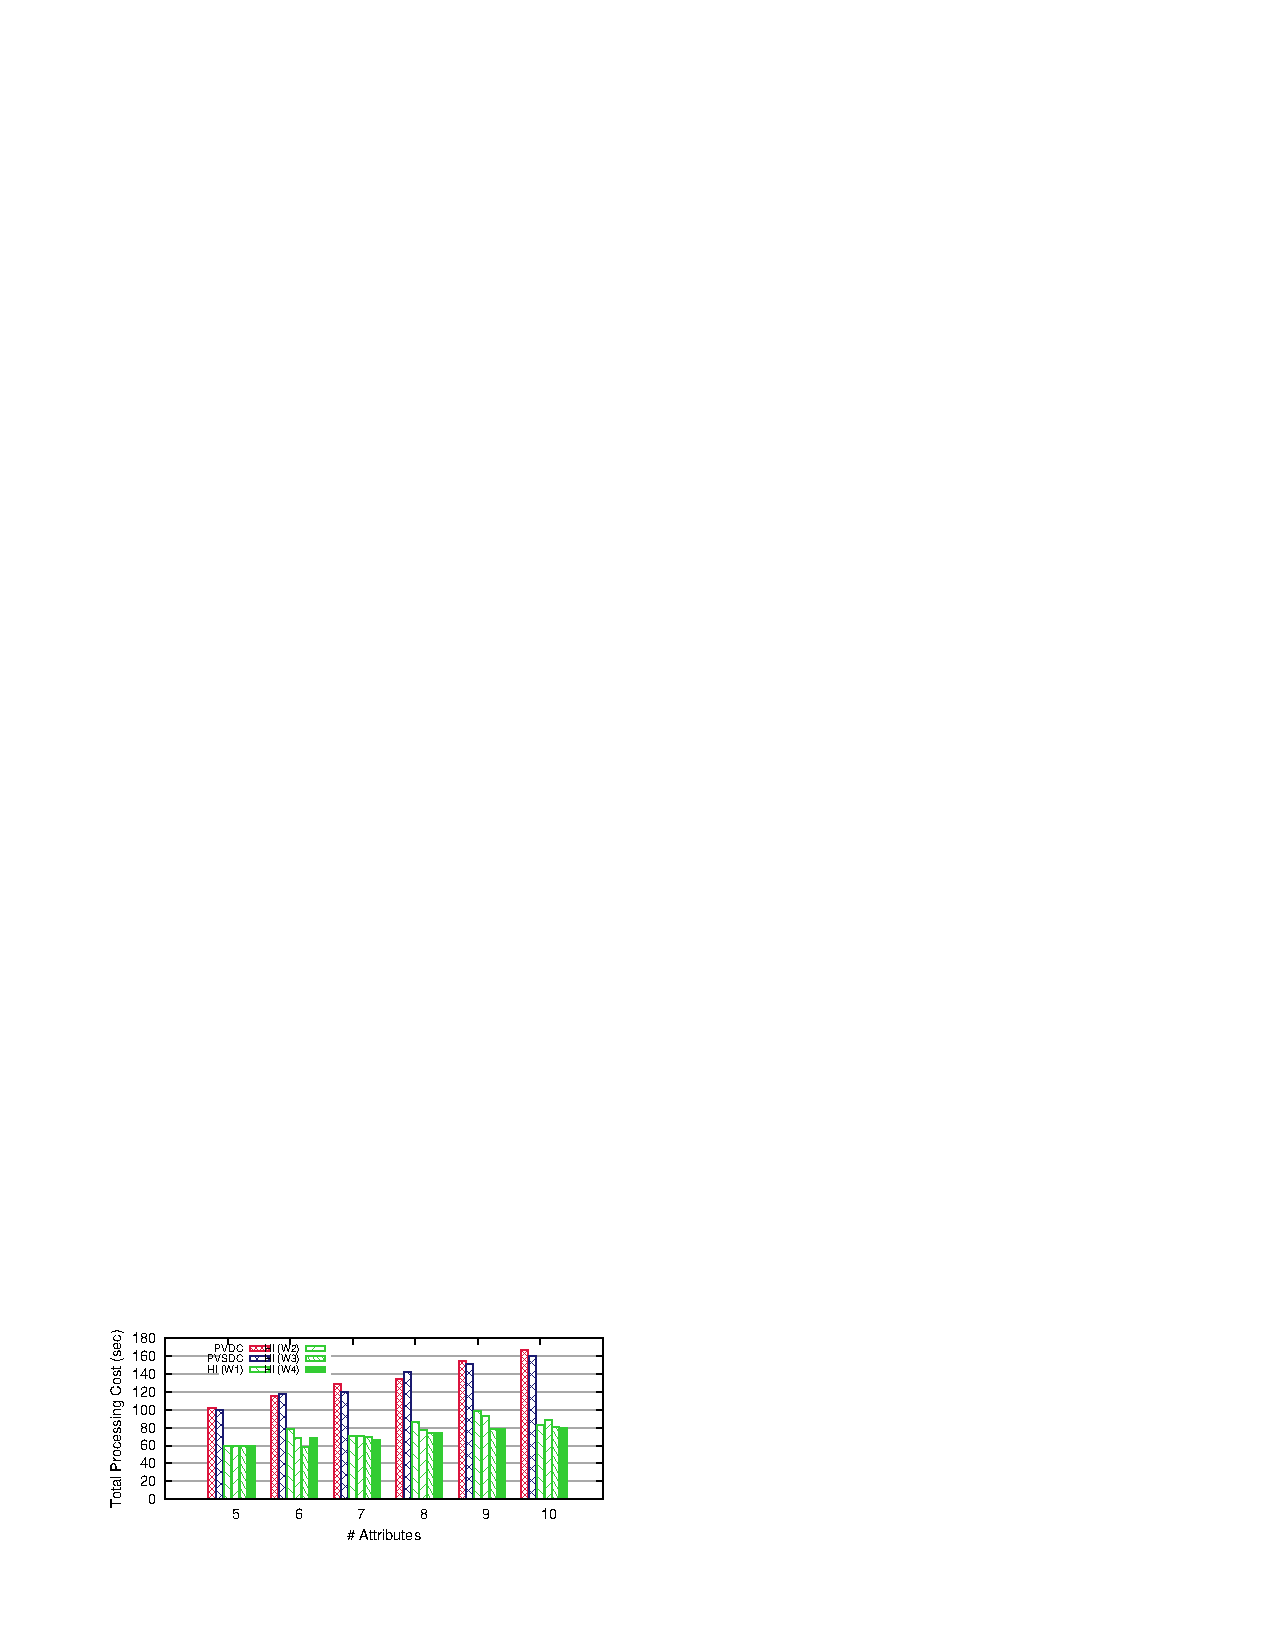
\includegraphics[trim=1.8cm 2.2cm 11cm 22cm]{Figures/holistic/skew_ma}
        }\vspace{-0.1 in}%
	\subfloat[Skewed Attributes - Periodic Values]{%
            \label{fig:skew_per_ma}
            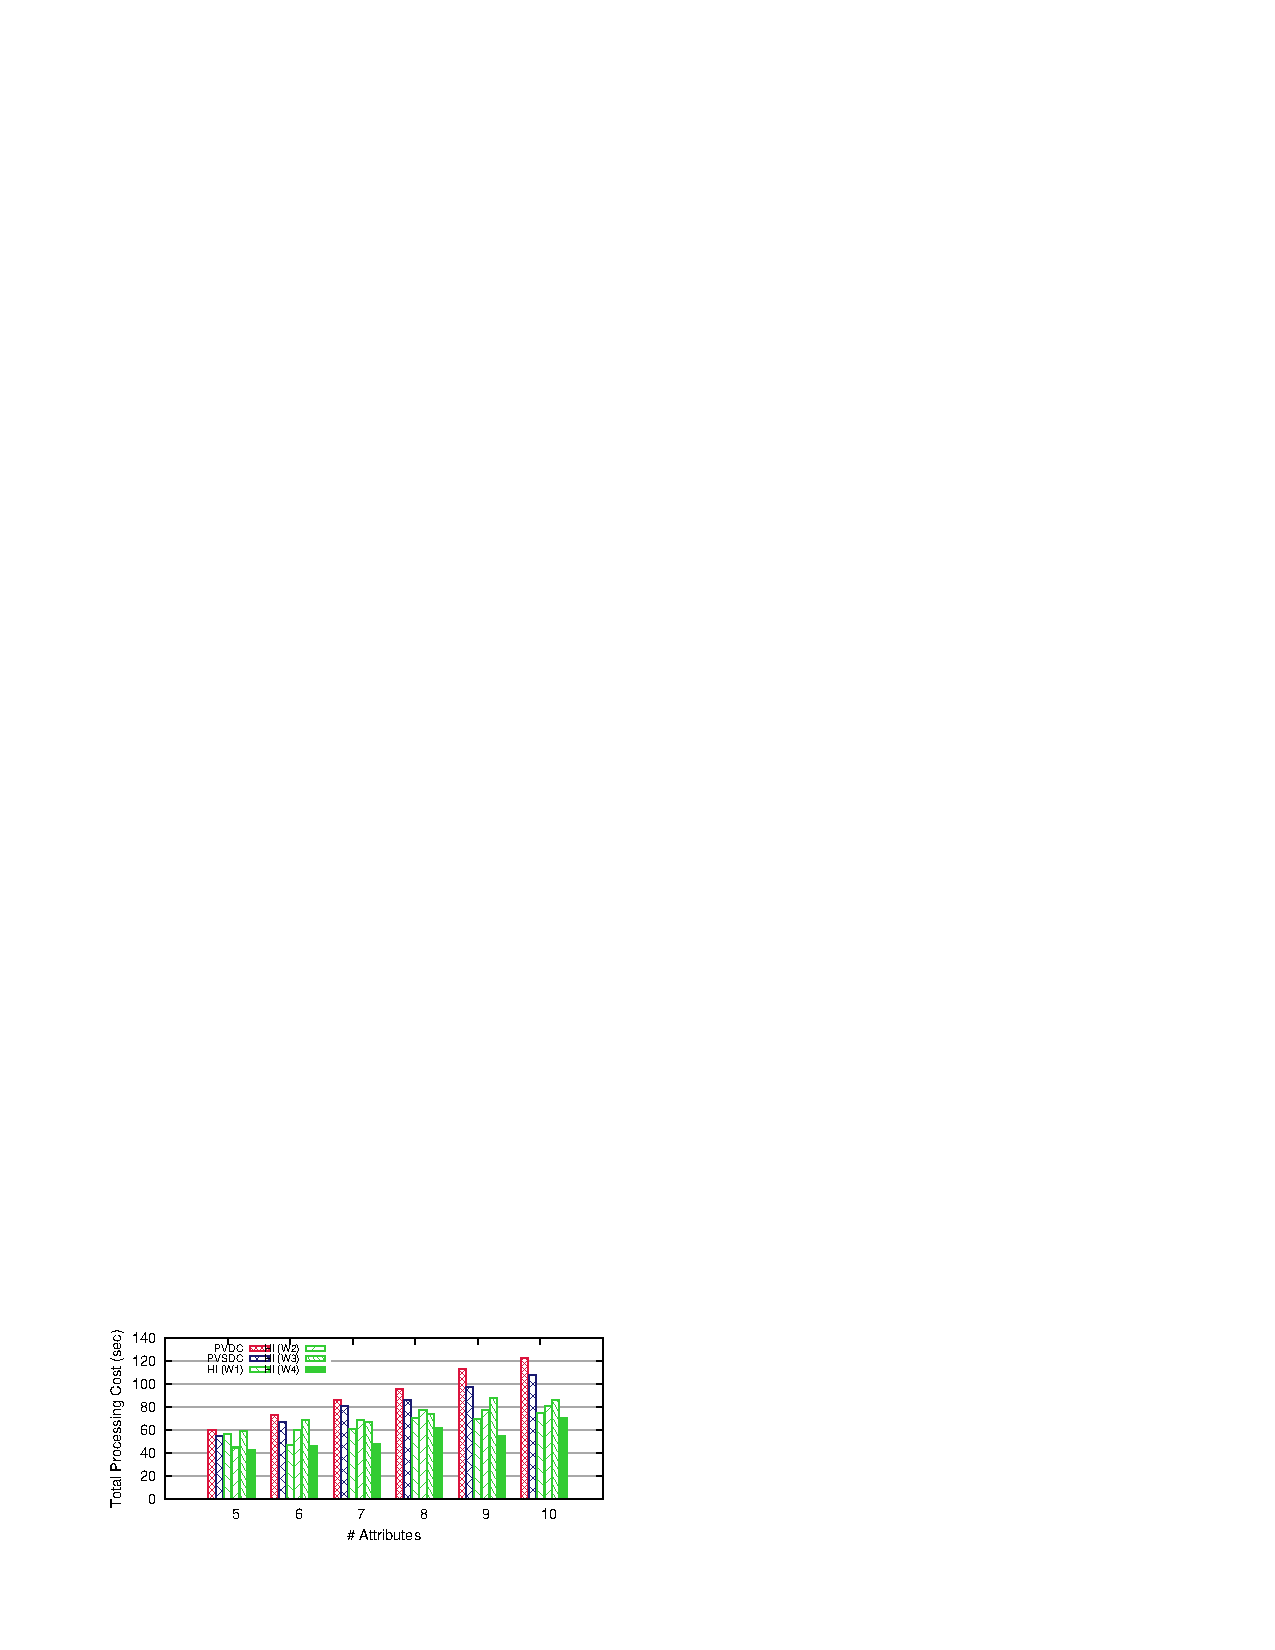
\includegraphics[trim=1.8cm 2.2cm 11cm 22cm]{Figures/holistic/skew_per_ma}
        }%\vspace{-0.2 in}
\vspace{-0.2 in}
   \caption{%
	More performance gains for holistic indexing as more attributes exist in a schema. All strategies have similar performance.
     }%
\vspace{-0.7 cm}
    \label{fig:hvsc}
    \end{center}
\end{figure*}

\subsection{Robustness}
\label{subsec:robustness}

In our next experiment we study how holistic indexing compares to parallel database cracking and parallel stochastic cracking
in terms of robustness.
We show that holistic indexing maintains the good properties of adaptive indexing by utilizing the available CPU resources more effectively.
Both holistic indexing and the parallel variants of adaptive indexing utilize all the available CPU cores.

We test four synthetic workloads.
Each workload consists of 10$^{3}$ queries on 10 attributes ($\sim$100 queries/attribute).
Each attribute consists of 2$^{30}$ uniformly distributed integers.
The queries follow a different pattern in each workload.
The first four subfigures in Figure~\ref{fig:rob1} depict those workload patterns. 
For each workload, the respective figure illustrates graphically 
how a sequence of queries touches the value domain of a single attribute.

Furthermore, we test holistic indexing in a real-life workload using data and queries from SkyServer \cite{SkyServer}.
SkyServer collects astronomical data  and the database can be accessed publicly by individual users and institutions.
We pose $10^4$ real user queries that have been logged by the project servers on the ``Photoobjall'' table.
The ``Photoobjall'' table consists of 1.2 Billion tuples.
All queries access the ``Ascension'' attribute and are posed in exactly the same chronological order they were logged.
The pattern the SkyServer queries follow is shown in Figure~\ref{fig:rob1}(e).

Figure~\ref{fig:stochastic} shows the results.
For each indexing method we report the total time needed to process all queries for each workload.



\textbf{Synthetic Workloads.}
In all synthetic workloads holistic indexing outperforms multi-core database cracking by a factor 2-10 depending on the workload.
Multi-core database cracking is strictly driven by query predicates, and thus, can leave large unindexed pieces to be reorganized by future queries.
For instance, in the sequential workload in Figure~\ref{fig:rob1}(d), each query cracks a column in a small piece and in a big piece, and then, a future query needs to crack the big piece again, resulting in a high cost.
Multi-core stochastic cracking solves these robustness issues by injecting one extra random cracking action for each user query in order to distribute cracking more evenly.
However, holistic indexing can materialize an even bigger advantage. This is because it is not restricted to perform auxiliary index refinement actions only during user queries but it can exploit all possible CPU cycles to refine the indices, resulting in many more actions taking place in parallel with user queries. 
Moreover, holistic indexing spreads the auxiliary index refinements across the entire value domain (by choosing random pivots) without leaving big unindexed pieces.
For example, in the skewed workload in Figure~\ref{fig:rob1}(b), both multi-core database cracking and multi-core stochastic cracking show a similar performance, because they restrict the index refinements to a small region of the domain according to user query predicates, i.e, from 800 million to $2^{30}$.
Future queries have to reorganize a big unindexed area, i.e., from 0 to 800 million; this area is already indexed in holistic indexing before the 800th query arrives.
Thus, holistic indexing prepares the physical design better for (ad-hoc) future queries.



\textbf{SkyServer.} 
The SkyServer workload in Figure~\ref{fig:rob1}(e) shows the pattern 
logged in SkyServer for queries using the ``right ascension'' attribute of the ``Photoobjall'' table.
We observe that the queries follow non-random patterns, i.e., they focus on a specific part of the sky before moving to a different part.
Figure~\ref{fig:stochastic} shows that holistic indexing manages to significantly outperform multi-core database cracking 
by inducing auxiliary index refinement actions in parallel with query processing without penalizing individual user queries.

Overall, in all workloads tested, holistic indexing not only maintains the nice properties of the parallel variants of database cracking and stochastic cracking, but it also enhances the behavior further by being able to exploit
all available CPU resources effectively for a better prepared physical design.

\begin{figure*}[t]
     \begin{center}

        \subfloat[TPC-H Query 1]{%
            \label{fig:random_pred}
            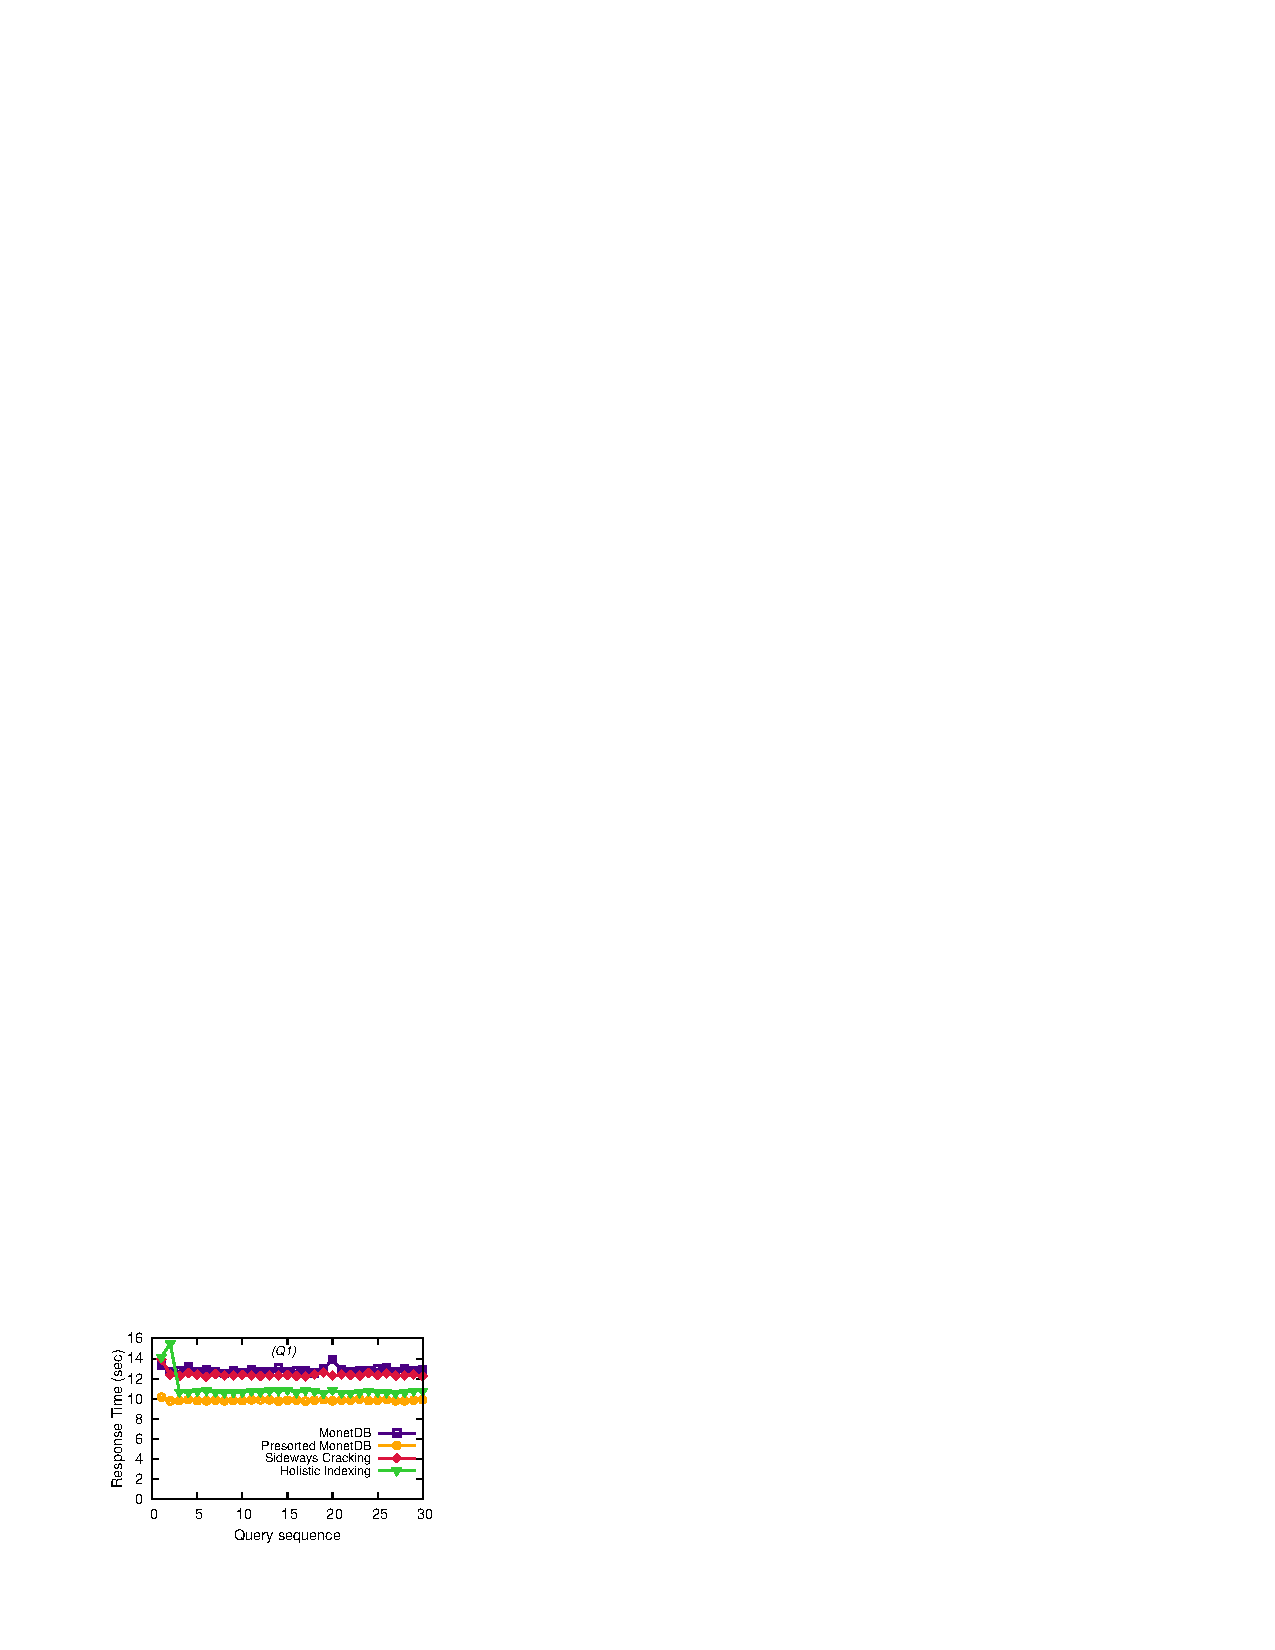
\includegraphics[trim=2cm 2cm 13.5cm 22.5cm]{Figures/holistic/tpch_q1}
        }%
	\subfloat[TPC-H Query 6]{%
            \label{fig:skew_pred}
            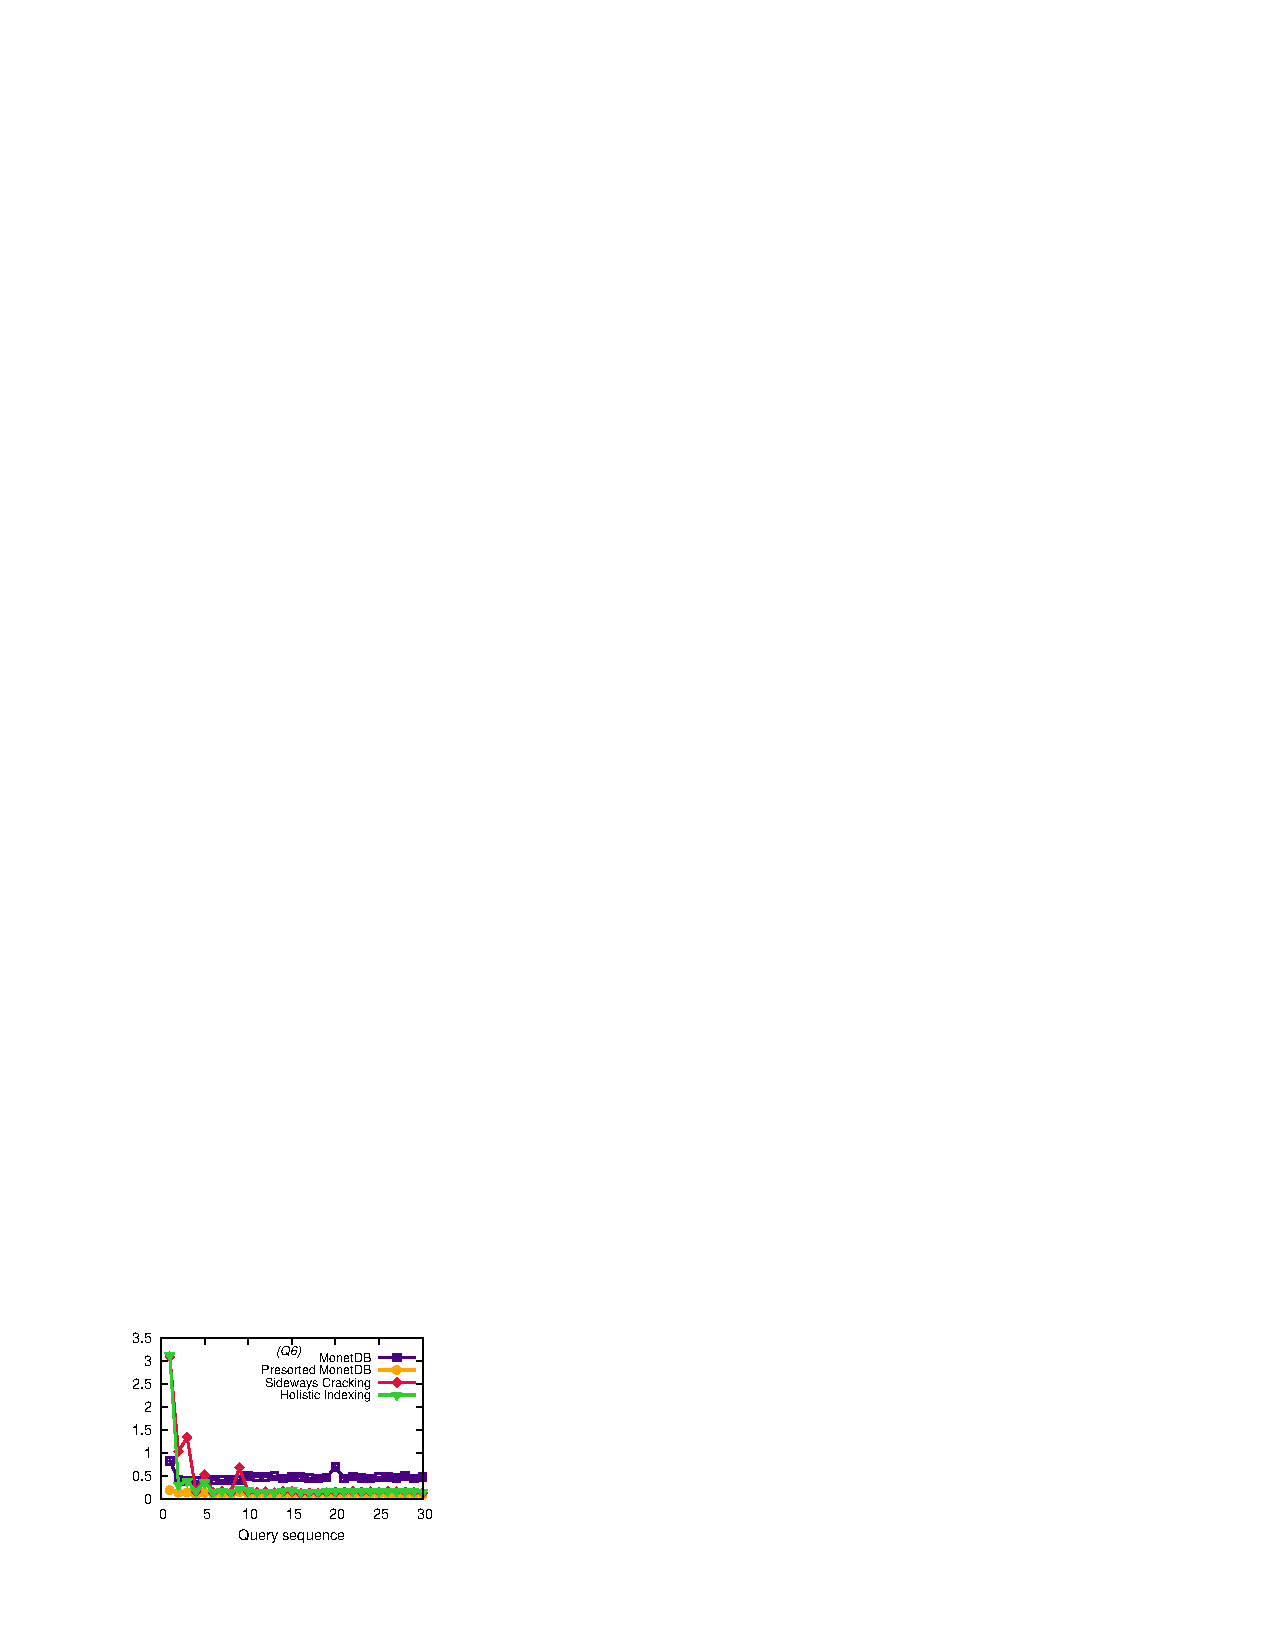
\includegraphics[trim=3cm 2cm 15cm 22.5cm]{Figures/holistic/tpch_q6}
        }%
      \subfloat[TPC-H Query 12]{%
           \label{fig:periodic_pred}
           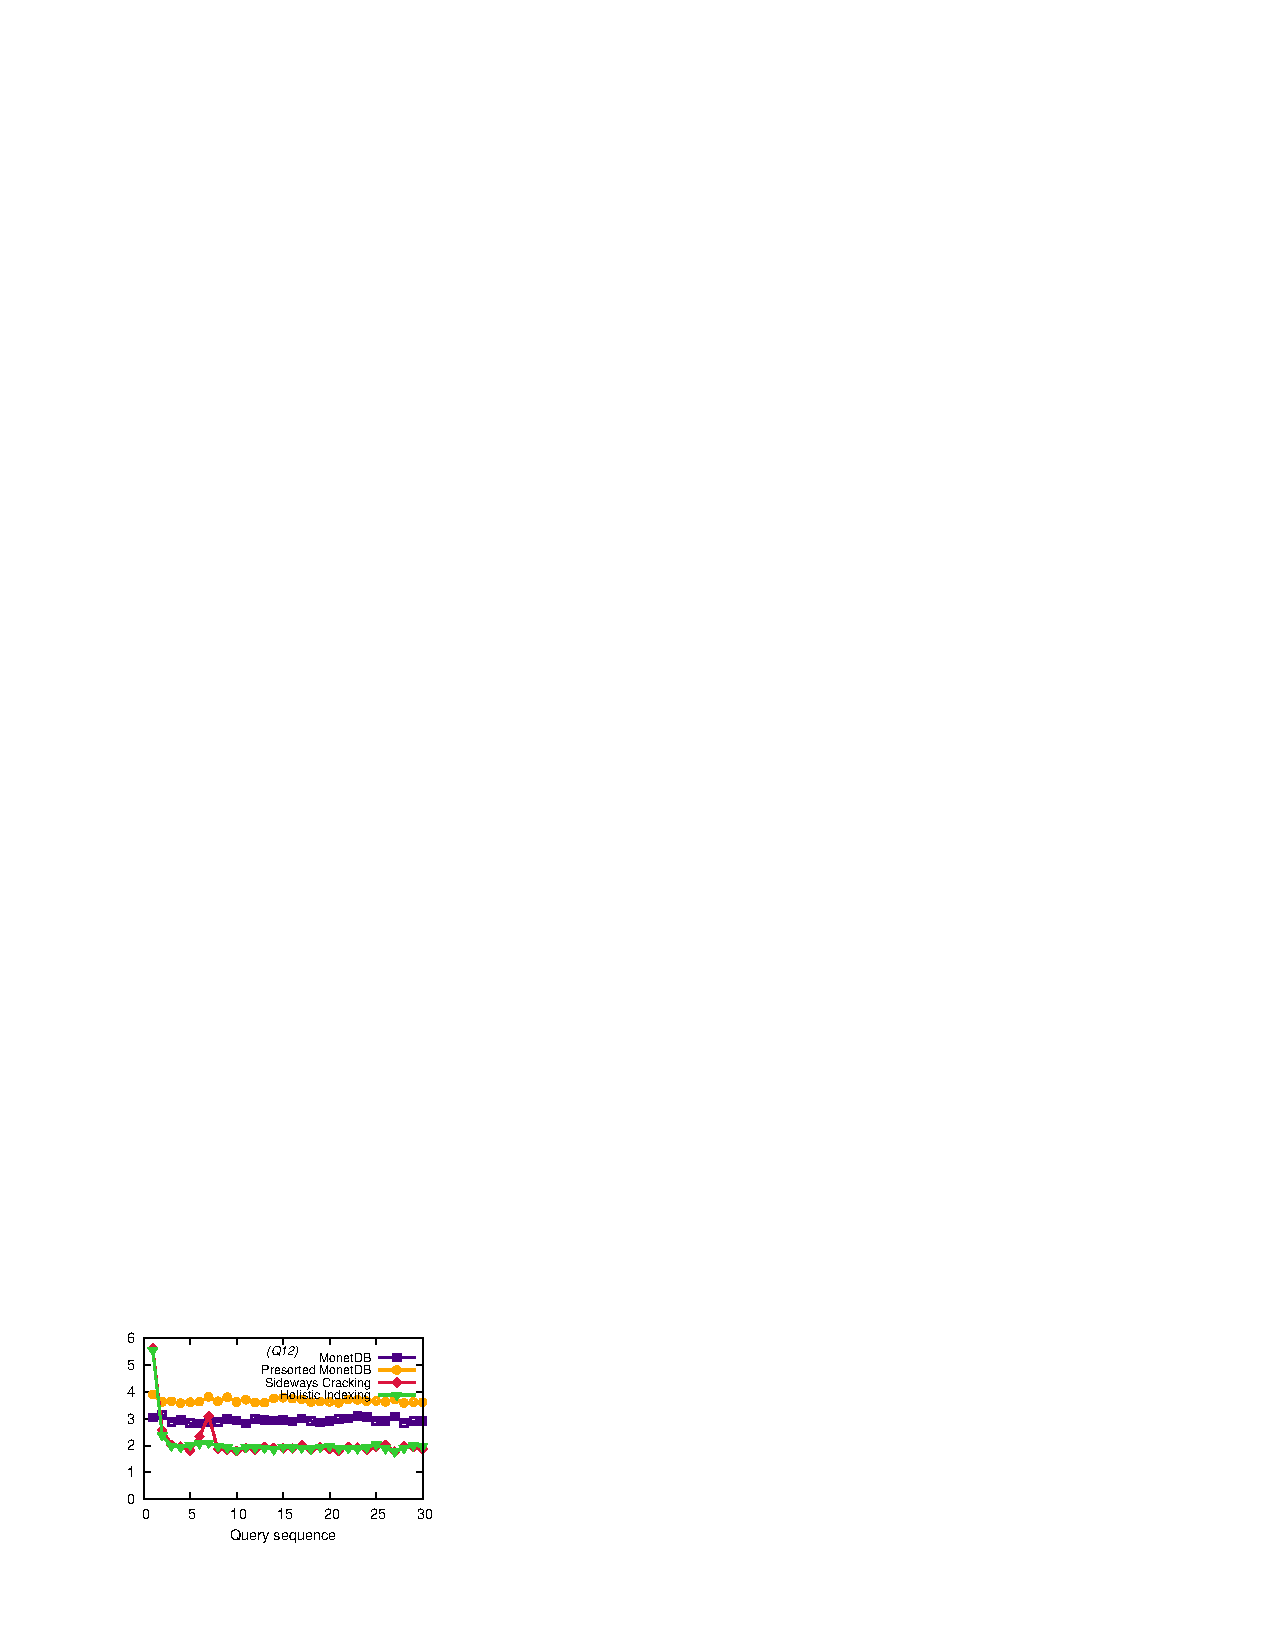
\includegraphics[trim=1.5cm 2cm 14cm 22.5cm]{Figures/holistic/tpch_q12}
        }%
\vspace{-0.25 in}
    \caption{TPC-H results (Scale Factor 10, ``pre-sorted'' times exclude pre-sorting costs; Q1,6,12: 8 sec).}
\vspace{-0.7 cm}
   \label{fig:tpch}
    \end{center}
\end{figure*}

%\newpage
\subsection{More Benefits with Complex Schemas}
\label{subsec:strategies}

In this experiment, we show that as the database schema becomes more complex by containing more attributes,
this brings more opportunities for holistic indexing to gain in performance;
more attributes make the indexing space bigger and thus any a priori decisions 
are even more prone to be wrong. In addition, we test the various strategies for choosing 
among the candidate indices and we show that indeed making random decisions is a robust approach. 

Here, we assume a gradually bigger database table which consists of 5-10 attributes.
Each attribute consists of $2^{30}$ uniformly distributed integers.
We fire select-project queries as in the previous experiments but this time we may query up to $X$
attributes in every run. 
Each query touches a single attribute and we vary the frequency with which each attribute is accessed, i.e.,
we run both a random workload where every attribute is evenly queried as well as a skewed workload
where some attributes are queried more than others.
For each workload we vary also the workload pattern followed by the queries.
Here, we present the results for random and periodic workload patterns.
For each case, we perform 10$^{3}$ queries.

We compare holistic indexing using one of the four strategies described in Section~\ref{subsec:design} against multi-core variants of database cracking and stochastic cracking.
Figure~\ref{fig:hvsc} shows the results;
for all cases, holistic indexing materializes a big benefit.
As the number of attributes in the database table grows, the performance benefit for holistic indexing increases. 
What happens is that holistic indexing makes sure to evenly spread
auxiliary index refinement actions across all attributes in parallel with user queries whenever free CPU
cycles are available. Then, future queries on those attributes can exploit this refined indexing. 
Compared to the case where we have a few attributes, having more attributes means that
more heavy indexing actions have to be performed overall in order to crack the columns into small pieces.
This allows holistic indexing to materialize a bigger benefit as it performs those actions in the background as opposed to 
only during user queries as in multi-core database cracking and multi-core stochastic cracking.

In addition, all index choosing strategies have similar performance on workloads where attributes are queried on random values (Figures~\ref{fig:hvsc}(a) and (c)), 
because indices are already fine-grained in such cases (even when some indices are refined more than others in a skewed workload).
However, in case of queries on periodic values (Figures~\ref{fig:hvsc}(b) and (d)) the random choice ($W4$) shows a clear performance benefit compared to the rest of the strategies, 
because it refines indices with big unindexed partitions,
and proves to be a robust design decision.


\begin{figure}[!htb]
\begin{center}
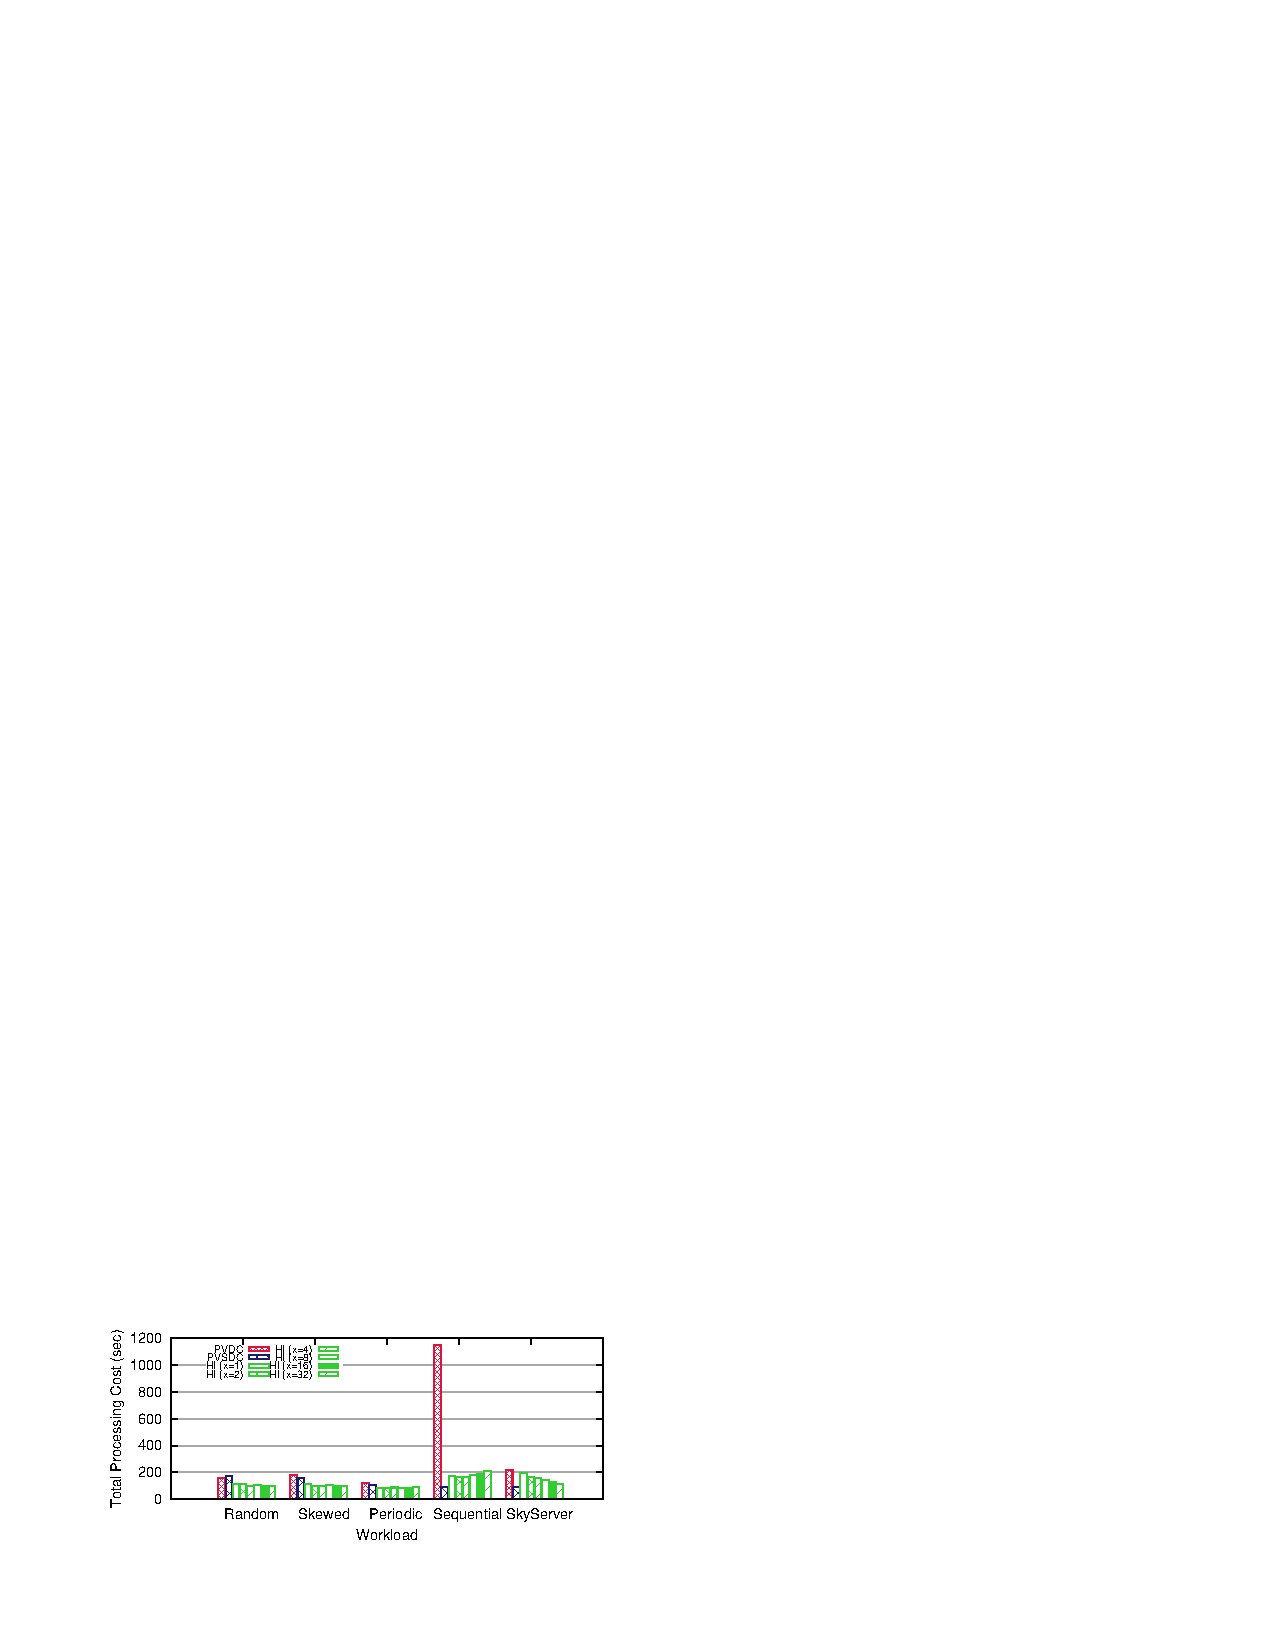
\includegraphics[trim=1.8cm 2cm 0cm 22.5cm]{Figures/holistic/cracks_number}
\vspace{-0.2 in}
\caption{Performance of holistic indexing improves while the number of index refinements $x$ increases.}
\vspace{-0.7 cm}
\label{fig:cracks_number}
\end{center}
\end{figure}


\subsection{Design Decisions}
\label{subsec:decisions}
%\vspace{-0.3cm}
\textbf{Holistic Worker Thread Refinements.}
In this experiment we demonstrate how the tuning parameter $x$, i.e., the number of index refinements per worker (Figure~\ref{fig:diagram}), affects the workload performance.
We test five workloads that consist of $10^{3}$ queries on a relation with 10 attributes as in Section~\ref{subsec:robustness} (Figure~\ref{fig:stochastic}).
We vary the number of index refinements each holistic worker thread does from 1 to 32 and we compare holistic indexing with multi-core variants of database cracking and stochastic cracking.
Figure~\ref{fig:cracks_number} shows the results.
The more index refinements each thread does, the bigger the benefit for holistic indexing because more pieces are created and thus future queries need to refine smaller pieces, touching less data.
However, when we increase the number of index refinements from 16 to 32, performance does not improve significantly, because in both cases indices converge very fast to optimal ones.
Thus, we use 16 as the number of index refinements that each holistic worker thread does in all our experiments.


\subsection{TPC-H}
\label{subsec:tpch}

In our next experiment, 
we evaluate holistic indexing on the standard database benchmark, TPC-H  \cite{tpch}.
We compare against offline indexing and relying on plain scans.
We use scale factor 10 and we test with Queries 1, 6, and 12.
For each query type, we created a sequence of 30 variations using the random query generator distributed with the benchmark. 
For offline indexing, we created the proper column-store projections by pre-sorting the data
depending on each query individually, i.e., we created the perfect projection for each query.
Specifically, for Queries 1 and 6 we created a copy of the Lineitem table sorted on the l\_shipdate attribute.
For Query 12 we created a copy of the Lineitem table sorted on the l\_receiptdate attribute.

Figure~\ref{fig:tpch} depicts the results.
For all cases, holistic indexing brings a significant advantage, resulting in a robust and stable 
performance across all queries.
The first query is slower as it creates the first adaptive indices which implies extra data copying
but after that all queries perform significantly better than plain MonetDB.
Holistic indexing matches offline  indexing without having to incur the high offline indexing cost
and without requiring any workload knowledge.
The pre-sorting cost for all queries is 8 seconds.
For Query 12, it turns out that pre-sorting does not help.
This happens because even though we may improve the selection by pre-sorting the Lineitem table,
it turns out we hurt the join between the Lineitem and the Orders table.
This is because in the base data, the Lineitem table contains 
the order date ordered and this can be exploited during the join.
With holistic indexing we do not face this problem, because the initial order changes only partially.


\subsection{Updates}
\label{subsec:updates}

So far we tested read-only workloads. 
In this experiment we demonstrate that holistic indexing maintains its nice properties  
in workloads where read-only queries interleave with write queries.
We test two scenarios.
In the first scenario (High Frequency Low Volume - HFLV), 10 inserts arrive every 10 queries.
In the second scenario (Low Frequency High Volume - LFHV), 100 inserts arrive every  100 queries.
In both scenarios the workload consists of 500 select project range queries on a single attribute $A$ and 500 insertions in total on a single attribute $A$.
While all queries are processed sequentially one after the other, the 11th query arrives 20 seconds after the 10th query resulting in idle time of 20 seconds in the system.
Attribute $A$ consists of 10$^{9}$ uniformly distributed integers.

\begin{wrapfigure}{l}{0.166\textwidth}
\begin{center}
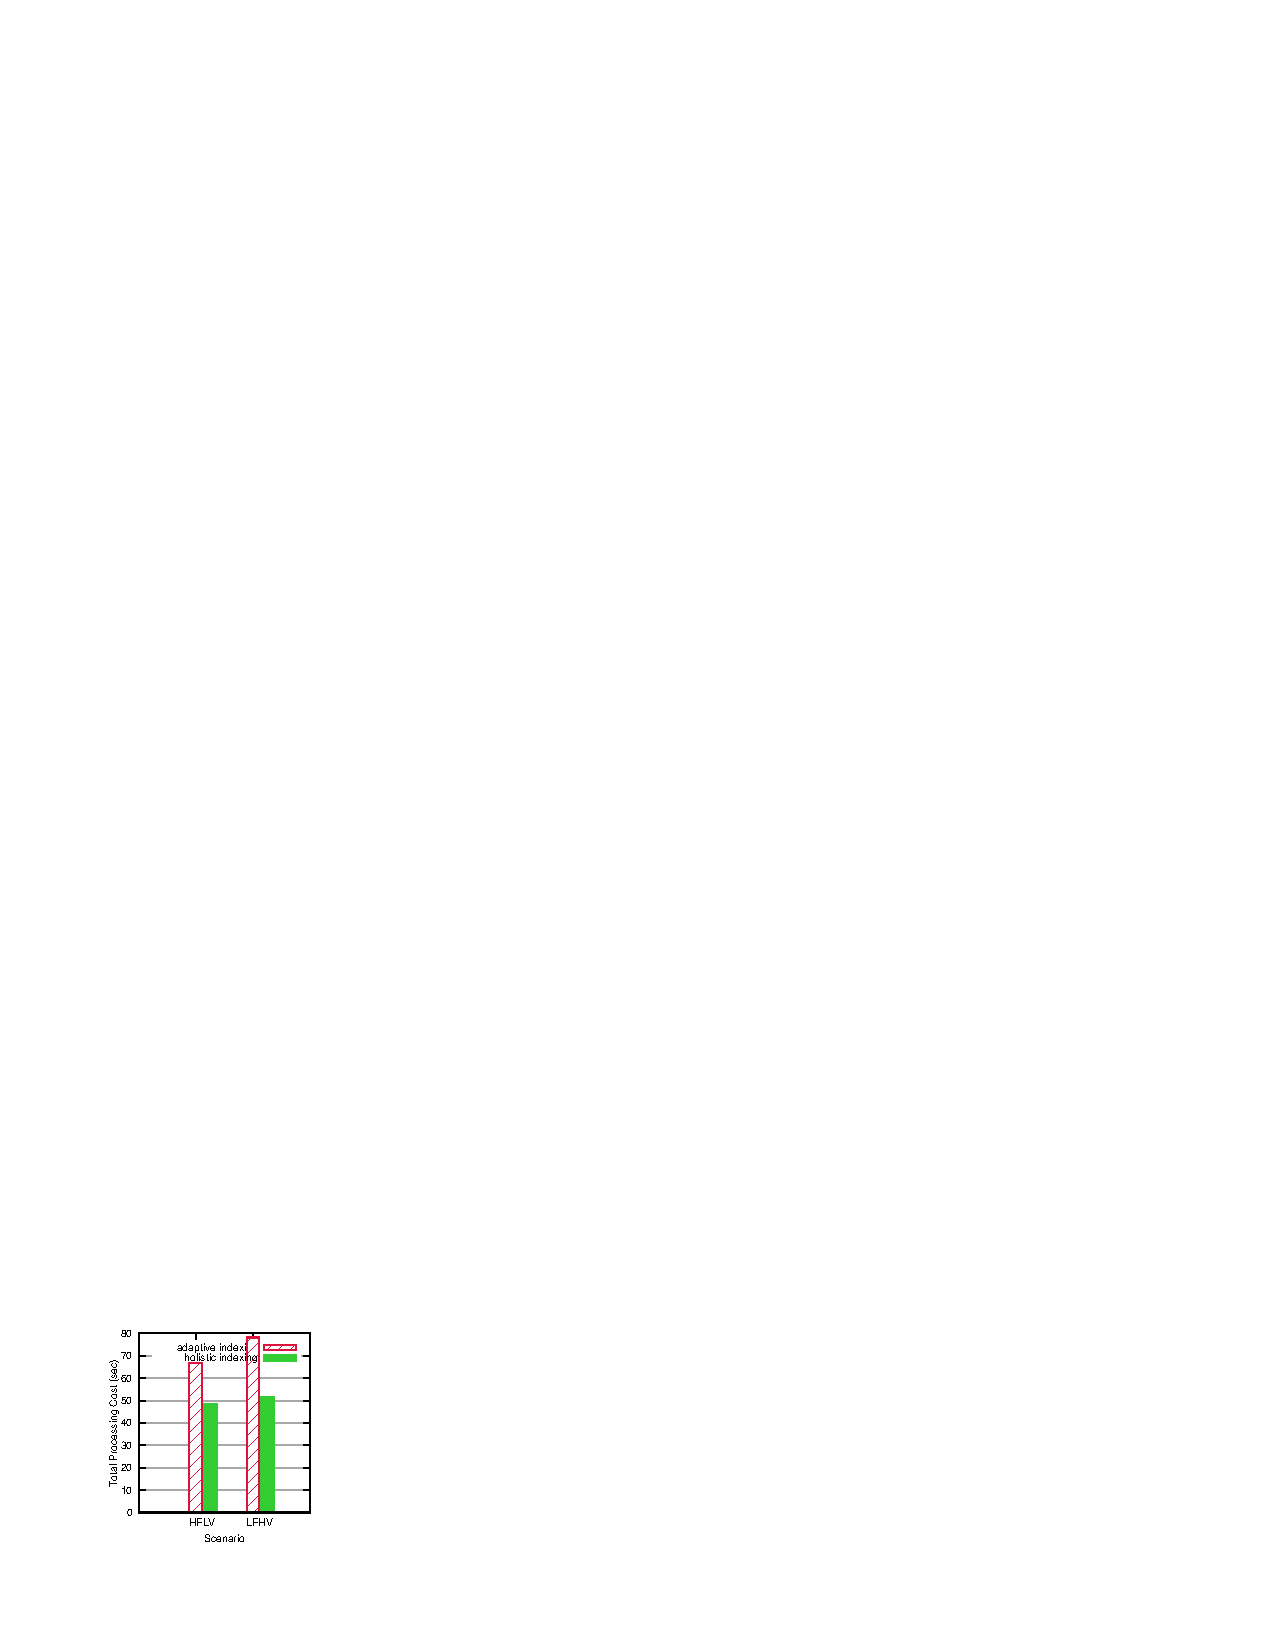
\includegraphics[trim=2.8cm 2cm 18cm 23.2cm]{Figures/holistic/updates}
\vspace{-0.1in}   %-0.1in
\caption{Updates.}
\vspace{-0.3in}
\label{fig:updates}
\end{center}
\end{wrapfigure}
Updates are temporarily stored in a pending insertions column.
We use the Ripple algorithm \cite{DBLP:conf/sigmod/IdreosKM07} in order to apply the updates;
a pending inserted value is merged with the original data if and only if the index partition, where the specific value belongs, is refined.
Thus, the merging process happens on-the-fly and maintains the information of the index.
In this experiment we test single-threaded adaptive indexing against holistic indexing with a single worker that refines the index only during idle time.
In holistic indexing,  
auxiliary  index refinement actions also cause  insertions to be merged. In this way, holistic indexing not only refines the indices but also consumes pending
 insertions, which speeds up future queries even more and all that by exploiting idle CPU resources in parallel with query processing.
Figure~\ref{fig:updates} shows the results.
In both scenarios, holistic indexing maintains its advantage over adaptive indexing;
it is not affected by updates and still provides roughly a 50\% improvement.

%\newpage
%\vspace{-0.1cm}

\subsection{Varying Number of Clients}
\label{subsec:varcpu}

\begin{wrapfigure}{l}{0.166\textwidth}
\begin{center}
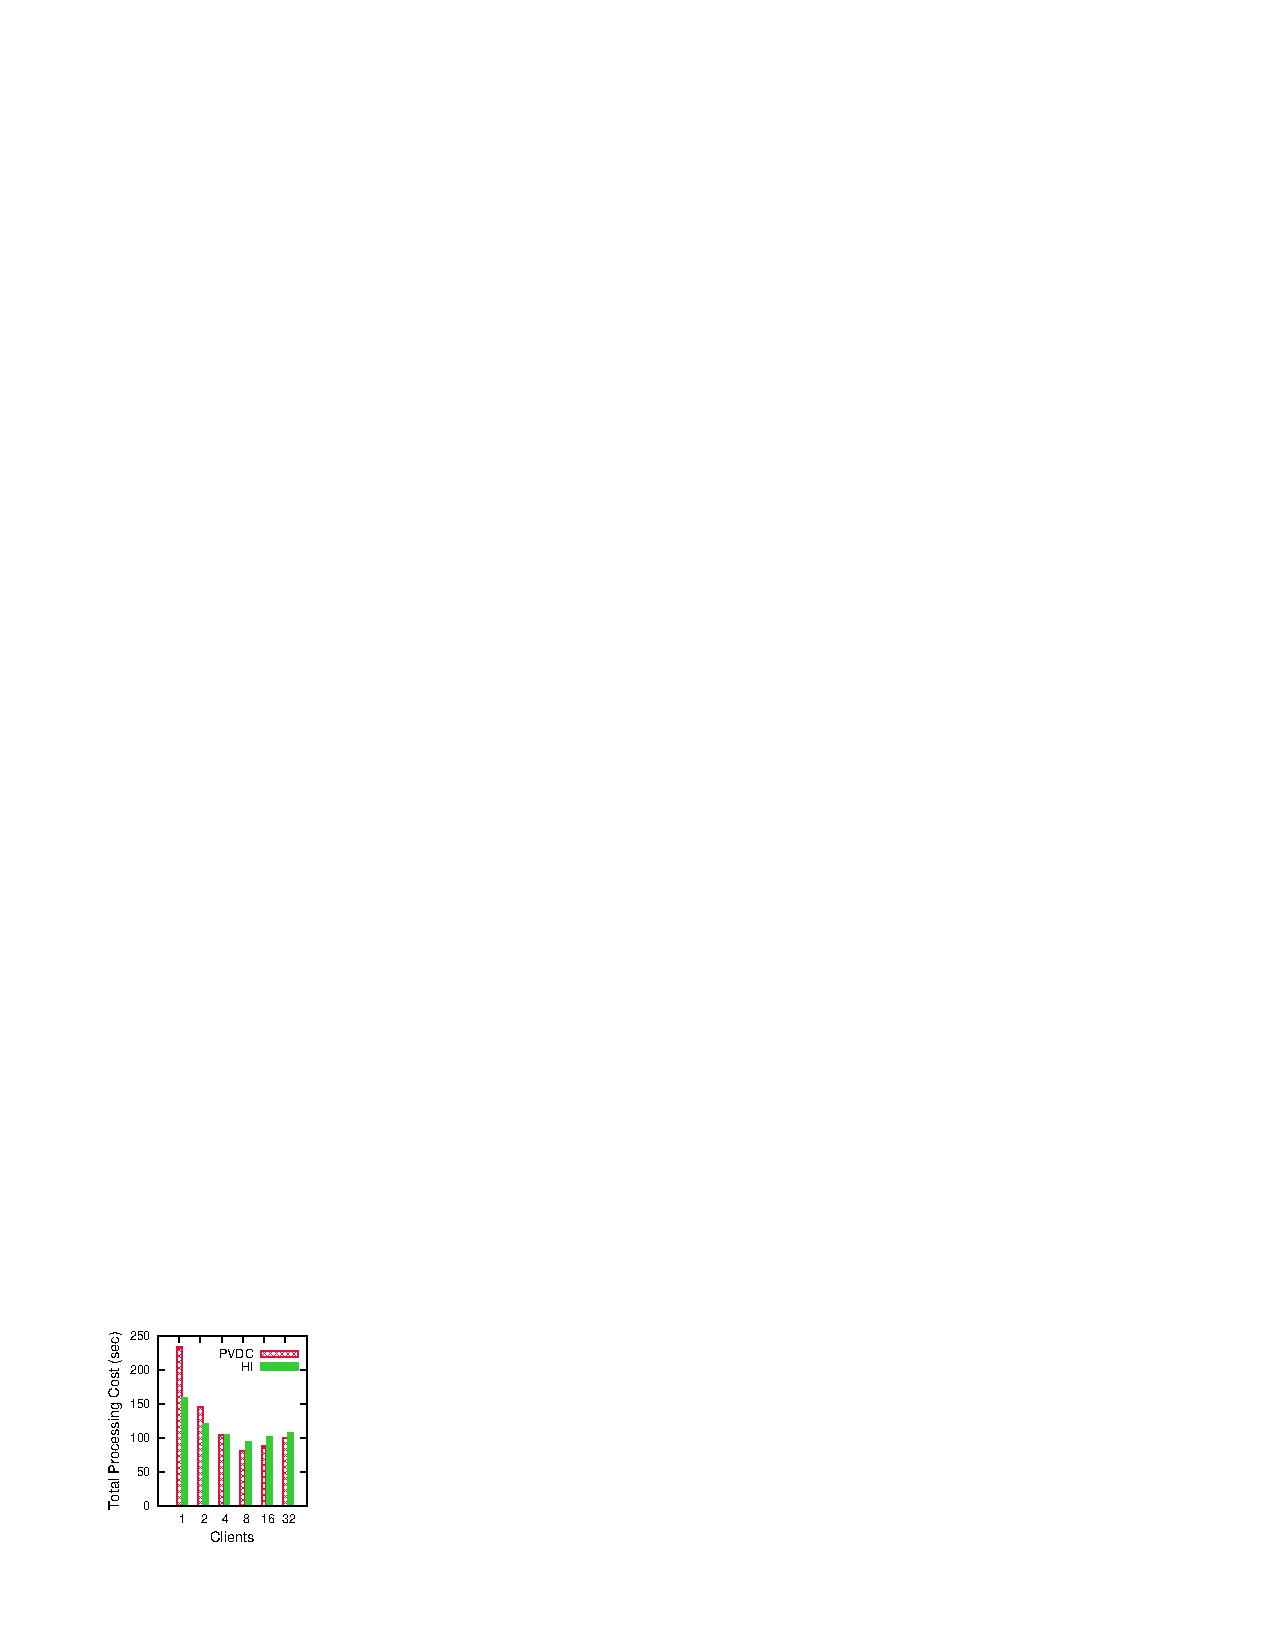
\includegraphics[trim=2cm 2cm 17cm 23cm]{Figures/holistic/threshold}
\vspace{-0.1in}
\caption{Varying number of clients.}
\vspace{-0.3in}
\label{fig:threshold}
\end{center}
\end{wrapfigure}
In this experiment we test the performance of holistic indexing with varying number of concurrent clients in the system.
Our workload consists of 1024 queries on a relation with 10 attributes.
We vary the number of concurrent clients between 1 and 32, where 32 is the number of CPU cores in our machine.
Figure~\ref{fig:threshold} shows that holistic indexing  brings a big benefit in case of a few clients.
The labels on top of the bars indicate the distribution of the available threads across user queries and holistic workers (similar  to Figure~\ref{fig:thread_distribution}).
When the number of clients increases, holistic indexing does not bring significant benefits, because it 
easily detects these cases as it monitors the CPU load continuously and so it is triggered only if the load is below a threshold.
%\newpage
